% !TeX encoding = UTF-8
% !TeX program = pdflatex
% !TeX spellcheck = en_US

%%%%%%%%%%%%%%%%%%%%%%%%%%%%%%%%%%%%%%%%%%%%%%%%%%%%%%%%%%%%%%%%%%%%%%%%%%%%%%%%%%%%%% PREAMBLE %%%%%%%%%%%%%%%%%%%%%%%%%%%%%%%%%%%%%%%%%%%%%%%%%%%%%%%%%%%%%%%%%%%%%%%%%%%%%%%%%%%%%%%%%%%%%%%%
\documentclass[english]{sapthesis}
\usepackage{microtype}
\usepackage{hyperref}
\usepackage{lipsum}
\usepackage{lscape}
\usepackage{siunitx}
\usepackage{makecell}
%\usepackage{subfig}
\usepackage{subcaption}
\usepackage[scale=0.9,copyright]{ccicons}
\usepackage[backend=biber,style=apa,sorting=nty]{biblatex}
\addbibresource{references.bib}
\hypersetup{pdftitle={Real Estate Inheritance and Wealth Inequality in Italy: An Empirical Analysis and Microsimulation of Tax Policy},pdfauthor={Paolo Sebastiani}}

%%%%%%%%%%%%%%%%%%%%%%%%%%%%%%%%%%%%%%%%%%%%%%%%%%%%%%%%%%%%%%%%%%%%%%%%%%%%%%%%%% TITLE %%%%%%%%%%%%%%%%%%%%%%%%%%%%%%%%%%%%%%%%%%%%%%%%%%%%%%%%%%%%%%%%%%%%%%%%%%%%%%%%%%%%%
\title{Real Estate Inheritance and Wealth Inequality in Italy: An Empirical Analysis and Microsimulation of Tax Policy}
\author{Paolo Sebastiani}
\IDnumber{1954447}
\course{Master's Degree in Economics}
\courseorganizer{Faculty of Economics}
\AcademicYear{2024/2025}
\advisor{Prof. Michele Raitano}
%\coadvisor{Dr. Sempronio}

%%%%%%%%%%%%%%%%%%%%%%%%%%%%%%%%%%%%%%%%%%%%%%%%%%%%%%%%%%%%%%%%%%%%%%%%%%%%% INFORMATION PAGE %%%%%%%%%%%%%%%%%%%%%%%%%%%%%%%%%%%%%%%%%%%%%%%%%%%%%%%%%%%%%%%%%%%%%%%%%%%%%%%
\examdate{21 October 2025}
\examiner{Prof. Giuseppe Ciccarone}
\examiner{Prof. Michele Raitano}
\examiner{Prof. Luigi Ventura}
\examiner{Prof. Jacob Louis Weisdorf}
\examiner{Prof. Cristiano Cantore}
\examiner{Prof. Dario Bonciani}
\examiner{Prof. Ana Maria Fagetan}
\authoremail{paoseba01@gmail.com}
\copyyear{2025}
\copyrightstatement{\raisebox{0.2ex}\copyright \quad 2025 Paolo Sebastiani. Licensed under \href{https://creativecommons.org/licenses/by-sa/4.0/}{CC BY‑SA 4.0} \raisebox{0.2ex}{\ccLogo} \raisebox{0.2ex}{\ccAttribution} \raisebox{0.2ex}{\ccShareAlike}}
\thesistype{Master thesis}


%%%%%%%%%%%%%%%%%%%%%%%%%%%%%%%%%%%%%%%%%%%%%%%%%%%%%%%%%%%%%%%%%%%%%%%%%% DEDICATION AND ABSTRACT %%%%%%%%%%%%%%%%%%%%%%%%%%%%%%%%%%%%%%%%%%%%%%%%%%%%%%%%%%%%%%%%%%%%%%%%%%%
\begin{document}
\frontmatter
\maketitle

\dedication{Dedicated to\\ ...}

\begin{abstract}
...
\end{abstract}


\tableofcontents
\mainmatter

%%%%%%%%%%%%%%%%%%%%%%%%%%%%%%%%%%%%%%%%%%%%%%%%%%%%%%%%%%%%%%%%%%%%%%%%%%%%%%% CHAPTER 1 %%%%%%%%%%%%%%%%%%%%%%%%%%%%%%%%%%%%%%%%%%%%%%%%%%%%%%%%%%%%%%%%%%%%%%%%%%%%%%%%%%%%
\chapter{Introduction}\label{ch:1}

%%%%%%%%%%%%%%%%%%%% SECTION 1.1 %%%%%%%%%%%%%%%%%%%%%%%%%%%
\section{Motivation: The Growing Importance of Wealth Inequality and Intergenerational Transfers in Italy}
In recent decades, the issue of economic inequality has returned to the forefront of academic and public discourse. Spurred by seminal works such as \cite{capital21century}, a growing body of research has shifted focus from income disparities to the more pronounced and persistent issue of wealth inequality. Wealth, defined as the total value of a household's assets minus its liabilities, offers a distinct and crucial perspective on economic well-being and opportunity, capturing the stock of resources available to a household beyond its periodic income flow. It provides economic security, enables investment in human capital, and confers social and political influence, as discussed in \cite{oecd2013chapter2}. Consequently, its unequal distribution has profound implications for social mobility, economic efficiency, and societal fairness.

The Italian context offers a particularly compelling case for the study of wealth inequality. Characterized by decades of sluggish economic growth and stagnant real wages (\cite{italydecline}), and one of the most rapidly aging populations in the world (\cite{agingpopulationitaly}), Italy's economic landscape has created an environment where accumulated capital and inherited assets play an increasingly dominant role over labor income in determining an individual's economic trajectory. The traditional pathways to wealth accumulation through savings from employment have weakened, making the starting point—the wealth of one's family—a more critical determinant of one's own financial success.

Within this framework, intergenerational transfers, particularly in the form of real estate, have become a central mechanism in the transmission of economic advantage across generations. Italy has historically maintained one of the highest home-ownership rates among advanced economies (\cite{italyhomeownership}), and real estate constitutes the largest single component of household wealth (\cite{Acciari2024}). For many Italian families, the primary residence is not only a place to live but also the most significant asset they will ever own and, crucially, pass on. As such, the inheritance of property is no longer a peripheral issue but a primary driver shaping the contemporary distribution of wealth (\cite{Cannari2008}). The transfer of these assets ensures that wealth remains concentrated within certain families, potentially ossifying class structures and limiting opportunities for those without a significant inheritance to look forward to.

This thesis, therefore, is motivated by the conviction that understanding the dynamics of real estate inheritance is fundamental to grasping the broader challenge of wealth inequality in Italy. By examining who inherits, what they inherit, and how these transfers affect the overall distribution of wealth, we can shed light on the persistence of inequality and evaluate potential policy interventions designed to foster a more equitable society. The analysis of inheritance tax policy, in particular, becomes a critical area of investigation in a country where such taxes are notably lower than in most other European nations.

%%%%%%%%%%%%%%%%%%%% SECTION 1.2 %%%%%%%%%%%%%%%%%%%%%%%%%%%
\section{Research Questions and Objectives}

Building upon the motivations outlined in the previous section, this thesis aims to provide a rigorous empirical investigation into the role of real estate inheritance in shaping wealth inequality in Italy. The study is guided by two central research questions, which move from a detailed descriptive and correlational portrait to a policy-oriented simulation:
\begin{itemize}
    \item \textit{What is the current socio-demographic and economic landscape of real estate inheritance in Italy, and which household characteristics are significantly correlated with it?} This question seeks to quantify the scale of wealth inequality, create detailed profiles of inheritor and non-inheritor households, and formally test the unconditional associations between key characteristics (e.g., parental education, age, geographical location) and the status of being an inheritor.

    \item \textit{What would be the potential redistributive impact of a reform of the Italian inheritance tax system?} Specifically, this question investigates the extent to which a revenue-neutral tax-and-transfer policy, leveraging increased taxation on large real estate inheritances, could mitigate the existing levels of wealth inequality.
\end{itemize}

To answer these research questions, the thesis sets out the following specific objectives:
\begin{itemize}
    \item To conduct a comprehensive descriptive and bivariate analysis of wealth distribution and real estate inheritance in Italy using the 2022 wave of the Bank of Italy's Survey on Household Income and Wealth (SHIW). This involves quantifying aggregate inequality, profiling distinct household groups, and using appropriate statistical tests to identify significant correlations.

    \item To develop and implement a static microsimulation model to evaluate the first-order effects of a hypothetical inheritance tax reform. This model will simulate the impact of the policy on the overall distribution of wealth, measuring changes in key inequality indicators such as the Gini index.
\end{itemize}


%%%%%%%%%%%%%%%%%%%% SECTION 1.3 %%%%%%%%%%%%%%%%%%%%%%%%%%%
\section{Contribution to the Literature}

This thesis contributes to the existing body of economic literature on wealth inequality and intergenerational transfers in several significant ways. While a substantial body of work has explored the theoretical underpinnings and empirical trends of wealth distribution, this study offers a targeted, timely, and methodologically robust analysis of the Italian case.

First, on an empirical level, this research provides an updated and granular analysis of the role of real estate in the intergenerational transmission of wealth in Italy. By utilizing the most recent available (2022) wave of the Bank of Italy's Survey on Household Income and Wealth (SHIW), it offers a contemporary snapshot of a landscape that may have shifted due to recent economic and demographic trends. This study's specific emphasis on real estate allows for a more nuanced understanding than analyses that treat inherited wealth as a single, homogenous category.

Second, the thesis makes a contribution through the depth and rigor of its descriptive approach. It moves beyond a simple presentation of summary statistics by integrating three layers of analysis: a quantification of aggregate inequality using formal indices and Lorenz curves; a detailed comparative analysis of distinct socio-economic groups based on housing tenure; and a formal bivariate analysis to statistically test the unconditional correlations between household characteristics and inheritance status. This multi-faceted descriptive framework provides a robust and comprehensive empirical foundation for the subsequent policy simulation.

Finally, and most significantly, this study contributes directly to the policy debate on inheritance taxation in Italy. The current Italian inheritance tax regime is one of the most lenient among advanced economies, yet there is a lack of recent, evidence-based research quantifying the potential redistributive effects of a reform. By simulating a specific, revenue-neutral tax-and-transfer scheme, this thesis moves beyond theoretical arguments to provide concrete, quantitative estimates of how such a policy could alter the distribution of wealth. These findings are intended to provide valuable, actionable insights for policymakers and stakeholders engaged in the discussion about tackling wealth inequality in Italy.


%%%%%%%%%%%%%%%%%%%% SECTION 1.4 %%%%%%%%%%%%%%%%%%%%%%%%%%%
\section{Structure of the Thesis}
The remainder of this thesis is structured as follows.

\paragraph{Chapter \ref{ch:2}} reviews the relevant theoretical and empirical literature. It covers theoretical frameworks of wealth inequality, empirical evidence on inheritance with a focus on Italy, and discusses the application of microsimulation models in policy analysis.

\paragraph{Chapter \ref{ch:3}} details the data and methodology. It introduces the Bank of Italy's Survey on Household Income and Wealth (SHIW) as the data source, defines key variables, outlines the microsimulation model, and acknowledges the study's limitations.

\paragraph{Chapter \ref{ch:4}} presents the initial empirical analysis, offering a descriptive portrait of wealth and inheritance in Italy. It examines the distribution of wealth, home-ownership rates, and provides a detailed profile comparing the socio-economic characteristics of inheritors and non-inheritors.

%\paragraph{Chapter \ref{ch:5}} moves to econometric analysis, identifying the key correlates of receiving a real estate inheritance. It details the model specifications, discusses estimation results and marginal effects to identify key factors, and includes robustness checks.

\paragraph{Chapter \ref{ch:5}} is dedicated to the microsimulation of a hypothetical inheritance tax reform. It outlines Italy's current tax system and a pre-tax baseline, then simulates a revenue-neutral tax-and-transfer scheme, presenting the quantified impact on inequality measures.

\paragraph{Chapter \ref{ch:6}} concludes the thesis, summarizing the main findings from the descriptive and microsimulation analyses. It then discusses policy implications and suggests avenues for future research.

%%%%%%%%%%%%%%%%%%%%%%%%%%%%%%%%%%%%%%%%%%%%%%%%%%%%%%%%%%%%%%%%%%%%%%%%%%%% CHAPTER 2 %%%%%%%%%%%%%%%%%%%%%%%%%%%%%%%%%%%%%%%%%%%%%%%%%%%%%%%%%%%%%%%%%%%%%%%%%%%%%%
\chapter{Literature Review}\label{ch:2}

This chapter reviews the key theoretical and empirical literature that forms the foundation for this thesis. The review is structured to move from a broad theoretical understanding of wealth inequality to the specific context of this study. Section \ref{sec:2.1} begins by outlining the major theoretical frameworks of wealth accumulation and distribution and the standard methods for its measurement. Section \ref{sec:2.2} narrows the focus to the microeconomic role of intergenerational transfers. We then ground the analysis in the specific Italian context in Section \ref{sec:2.3} by examining recent empirical evidence on inheritance and wealth disparities in the country. Subsequently, Section \ref{sec:2.4} reviews the economic literature on inheritance taxation, covering both theoretical debates and empirical findings. Finally, Section \ref{sec:2.5} introduces the microsimulation modeling approach, which provides the methodological framework for the policy simulation in this thesis.

%%%%%%%%%%%%%%% SECTION 2.1 %%%%%%%%%%%%%%%%%%
\section{Theoretical Frameworks of Wealth Inequality} \label{sec:2.1}

\subsection*{Capital Accumulation and Wealth Distribution}
The relationship between capital accumulation and wealth distribution is a cornerstone of economic thought, rooted in the work of classical economists like \cite{ricardo1817} and \cite{marxkapitalvol1}. Marx, in particular, argued that capital accumulation inherently concentrates wealth, a prediction revisited in modern studies (\cite{Bartels2025}).

The neoclassical growth model, developed by \cite{solow1956}, provided a crucial theoretical benchmark. In its standard formulation, the model predicts a steady state with constant capital-output ratios and income shares, implying that persistent increases in wealth inequality must be driven by mechanisms beyond basic accumulation, such as shocks or agent heterogeneity.

To address these limitations, modern macroeconomic research shifted to heterogeneous agent models where precautionary savings against idiosyncratic risk generate significant wealth dispersion. More advanced frameworks incorporating mechanisms like capital income risk (\cite{Benhabib2015}) or employing continuous-time approaches to model wealth dynamics (\cite{Achdou2021}) have been developed to better align with empirical data. However, a common finding is that standard models often struggle to replicate the extreme wealth concentration observed at the very top of the distribution without such additional features (\cite{DeNardi2015}).

Contemporary quantitative models incorporate additional features to generate more realistic outcomes. \cite{Quadrini1999} highlighted the role of entrepreneurship, while \cite{Benhabib2019} identified three key ingredients to match the US wealth distribution: skewed labor earnings, heterogeneous saving rates, and stochastic idiosyncratic returns to wealth.

A highly influential recent contribution is from \cite{capital21century}, who proposed the inequality $r>g$. They argue that if the return on capital ($r$) consistently exceeds the economic growth rate ($g$), existing wealth compounds faster than income, increasing wealth concentration. This dynamic suggests inherited wealth will become increasingly dominant. Extensive empirical work by Piketty, Saez, and Zucman supports this claim (\cite{SaezZucman2016}; \cite{PikettyYangZucman}).

This framework is not without its critics. \cite{Rognlie2015} found that the recent rise in the U.S. capital share is almost entirely due to the housing sector, questioning the generality of the mechanism. Others, like \cite{Stiglitz2012}, argue that this focus on mechanistic forces overlooks the critical role of institutions and rent-seeking. This body of work collectively shows that while capital accumulation is a fundamental driver of inequality, its impact is mediated by risk, behavior, and institutional context.

\subsection*{Measures of Inequality}
The empirical study of inequality requires a clear conceptual and methodological framework for its measurement. A primary distinction must be made between income, a flow of resources over a period, and wealth, a stock of assets at a point in time. While related, they capture different dimensions of economic well-being, with wealth typically being far more concentrated than income. 

Theoretically, the most comprehensive measure of economic well-being is \textit{full income}, defined as the level of consumption a household can sustain without depleting its net worth (\cite{Simons1938}). In empirical research, this concept is often proxied by \textit{equivalized disposable income}. This measure encompasses all market-based earnings and public transfers, net of taxes, and is adjusted for household size to allow for meaningful comparisons (\cite{CanberraGroup}).

\textit{Net wealth} (or \textit{net worth}), on the other hand, is defined as total assets minus liabilities. Official sources and distributional accounts specify that \textit{personal or household wealth = (sum of financial + non‐financial assets) minus (financial liabilities)}. This includes housing, business capital, stocks, bonds, pension entitlements, etc., less mortgages, loans and other debts.

To quantify the dispersion of wealth and income, a range of statistical indices are employed, each with specific properties. The most widely used summary measure is the \textit{Gini} coefficient, derived from the Lorenz curve, which captures overall inequality in a single value ranging from $0$ (perfect equality) to $1$ (maximal inequality). Its scale and population independence make it a standard tool for international comparisons (\cite{Ginicoeff}).

While the Gini coefficient provides a holistic view, much of the contemporary literature focuses on the concentration of resources at the top of the distribution. Top income and wealth shares, such as the share held by the richest 1\% or 10\%, are frequently used to track the evolution of economic elites. These are complemented by percentile ratios (e.g., $P90/P10$ or $P90/P50$), which measure the gap between different points of the distribution.

More complex measures include the parametric family of measures based on information entropy, the \textit{Generalized Entropy indices $(GE(\alpha))$}, where the most used are with $\alpha = 0,1,2$.
A key advantage of these indices is their decomposability, which allows total inequality to be partitioned into within-group and between-group components, offering deeper analytical insights.

Finally, the \textit{Atkinson index} allows for the incorporation of an explicit inequality aversion parameter, making normative judgments about social welfare transparent.

A detailed description of all these measures can be found in \cite{Atkinsonchapter2}.

%%%%%%%%%%%%%%%%%%%% SECTION 2.2 %%%%%%%%%%%%%%%%%%%%%%%%%
\section{The Role of Intergenerational Transfers}\label{sec:2.2}
Beyond macroeconomic accumulation, the transmission of wealth is fundamentally a microeconomic process driven by intergenerational transfers. Theoretical literature offers several explanations for bequests. Foundational altruistic models (\cite{Barro1974}); \cite{BeckerTomes1979}) posit that parents leave bequests because they care about their children's well-being, creating a direct link for the persistence of economic status. Alternative theories suggest more strategic motives, such as using inheritance to elicit care from children (\cite{Bernheim1985}) or as part of an implicit family risk-sharing arrangement (\cite{Kotlikoff1981}). Other models distinguish intentional transfers from accidental bequests arising from lifespan uncertainty (\cite{Cremer2010}).

Empirically, the importance of these transfers in wealth accumulation is well-documented (\cite{GaleScholz1994}). However, their effect on wealth inequality is debated. Many studies for the U.S. and Scandinavian countries find an equalizing effect, as inheritances provide a larger relative wealth boost to less affluent heirs, thus reducing overall inequality measures (\cite{Elinder2018}; \cite{Wolff2014}).

This effect is not universal. Research by \cite{Boserup2016} shows that bequests can increase absolute wealth dispersion (while reducing relative inequality). Most relevant for this thesis, a cross-country study by \cite{Palomino2021} finds that intergenerational transfers and family background contribute to wealth inequality.

From a long-run perspective, \cite{PikettyZucman2014} show that the economic share of inherited wealth is on a rising trend after a mid-20th century decline. This resurgence, linked to the $r>g$ dynamic, suggests intergenerational transfers are becoming a more dominant factor in shaping wealth concentration in advanced economies.

%%%%%%%%%%%%%%%%%%%% SECTION 2.3 %%%%%%%%%%%%%%%%%%%%%%%%%
\section{Empirical Evidence on Inheritance and Wealth Distribution in Italy}\label{sec:2.3}
The Italian case presents a unique landscape for studying wealth inequality, characterized by high aggregate wealth-to-income ratios alongside significant and growing disparities. Foundational empirical work by \cite{Acciari2024}, using novel inheritance tax data, reveals a substantial increase in wealth concentration between 1995 and 2016. Their findings show the share of total net wealth held by the richest 1\% rose from 16\% to 22\%, while the share of the bottom 50\% of the population collapsed from 11.7\% to just 3.5\% over the same period. This sharp divergence marks Italy as having one of the most pronounced declines in the wealth share of the lower half among developed nations.

A primary driver of this dynamic is the significant role of intergenerational transfers. Using data from the Survey of Household Income and Wealth (SHIW), \cite{Cannari2008} establish that bequests and gifts are a cornerstone of wealth accumulation in Italy. They estimate that the share of current net worth directly attributable to transfers (in 2002) ranges from 30\% to 55\%, depending on the methodology, and note that this share has been increasing over time. These transfers are also highly concentrated, with the top decile of households receiving approximately three-quarters of all inherited wealth. More recent findings from \cite{Acciari2024} corroborate this, showing that the annual flow of inheritances and gifts has doubled to constitute 14\% of national income, with these transfers becoming increasingly concentrated at the top of the distribution.

This high concentration of inherited wealth translates directly into low intergenerational mobility. Using SHIW data and an imputation methodology, \cite{bloiseraitano} provide some of the first estimates of intergenerational wealth persistence in Italy. Their findings point to a highly immobile society, with a preferred \textit{intergenerational wealth elasticity} (IWE) of 0.451 and a \textit{rank-rank slope} of 0.349. These figures are comparable to those found for the United States, indicating that parental wealth is a very strong predictor of a child's future economic standing.

This picture of low mobility is consistent across different measures of economic well-being, though estimates vary. Using administrative tax data to study income, \cite{Acciari2022} find that Italy is somewhat more mobile than previously estimated from survey data, but still exhibits significant persistence. Crucially, both their work and that of \cite{bloiseraitano} uncover stark geographical divides, with a pronounced North-South gradient where the southern regions are characterized by significantly lower mobility. This regional heterogeneity is a defining feature of inequality in Italy, suggesting that the "lottery of birth" is compounded by geography.

%%%%%%%%%%%%%%%%%%%% SECTION 2.4 %%%%%%%%%%%%%%%%%%%%%%%%%
\section{The Economics of Inheritance Taxation}\label{sec:2.4}

\subsection*{Theoretical Justifications and Efficiency Costs}
The normative debate over taxing wealth transfers is rooted in a fundamental trade-off between equity and efficiency, and different theoretical frameworks yield starkly opposing conclusions. 

The theoretical case against inheritance taxation rests on seminal work in optimal capital income taxation, which treats bequests as a form of capital accumulation. In influential papers, \cite{Chamley1986} and \cite{Judd1985} used infinite-horizon models with dynastic altruism to argue that the optimal long-run tax rate on capital income is zero. The core intuition is that any constant, positive tax on capital returns creates an economic distortion that compounds over time. For an infinitely-lived dynasty, this compounding wedge between the pre- and post-tax return to saving makes the tax exceptionally inefficient in the long run. The policy implication is to tax capital heavily in the short term (when the stock is fixed and the tax acts like a lump-sum levy) but to announce a credible commitment to phase the tax out over time.

This powerful "zero capital tax" result, however, relies on a series of strong assumptions that have been challenged by subsequent literature. The classic \cite{AtkinsonStiglitz1976} theorem, for instance, suggests that if a non-linear income tax can optimally address inequality in earning ability, and if preferences are separable between labor and consumption, then there is no need for additional taxes on commodities. In this context, an inheritance can be seen as future consumption, implying no need for a separate tax. However, as \cite{Pikettyoptimaltax} argue, this logic fails when inequality is bi-dimensional. The presence of inheritances means that lifetime resources are determined not just by earnings but also by transfers, breaking the conditions of the Atkinson-Stiglitz theorem and creating a clear role for inheritance taxation as a distinct policy instrument.

Furthermore, the desirability of wealth transfer taxation depends critically on the underlying motive for leaving a bequest, a point explored in detail by \cite{CremerPestieau} and \cite{Batchelder2010}. If bequests are purely accidental—the result of precautionary savings in a world of lifetime uncertainty—then taxing them is highly efficient, as the tax does not distort the original saving decision. Conversely, if bequests are purely altruistic, as assumed in the Chamley-Judd framework, then taxes directly distort the saving choices of parents who care about their children's welfare. A third category is "joy-of-giving" or "warm-glow" bequests, where individuals derive utility from the act of giving itself. In this case, the bequest is akin to a form of consumption for the donor and, from a tax theory perspective, should be included in the tax base. A final motive is exchange-based, where bequests are effectively payments for services; such transfers should be treated as taxable income for the recipient.

The modern "sufficient statistics" approach, developed by \cite{Pikettyoptimaltax}, synthesizes these competing arguments. This framework shows that the optimal inheritance tax rate can be expressed as a formula depending on empirically estimable parameters rather than unobservable primitives like bequest motives. The formula transparently captures the equity-efficiency trade-off: the optimal tax rate is lower when the elasticity of bequests to taxation is high (the efficiency cost), and higher when inherited wealth is highly concentrated and society has a strong preference for redistribution (the equity gain). This approach nests the Chamley-Judd result as the special case where the long-run elasticity of aggregate bequest flow (i.e., aggre-
gate capital accumulation) to the net-of-bequest-tax rate (i.e., \textit{1 - tax on bequest}) is infinite, but it demonstrates that for finite, realistic elasticities, the optimal tax rate is positive and can be substantial.


%%%%%%%%%%%%%%%%%%%% SUBSECTION 2.4.2 %%%%%%%%%%%%%%%%%%%%%%%%%%
\subsection*{Empirical Effects of Inheritance Tax on Wealth Inequality}
The empirical literature on the impact of inheritance taxation on wealth inequality presents a complex and often counter-intuitive picture. While inheritances themselves are highly concentrated, a significant body of research suggests that, at the moment of transfer, they tend to reduce relative measures of wealth inequality, such as the Gini coefficient. This seemingly paradoxical result is driven by the fact that less wealthy heirs, while receiving smaller inheritances in absolute terms, receive amounts that are much larger relative to their pre-existing wealth.

Studies using administrative data from Scandinavian countries have been particularly influential in demonstrating this effect. \cite{Elinder2018}, using Swedish population register data, find that inheritances mechanically reduce the Gini coefficient for wealth by approximately 7\% upon receipt. This equalizing effect occurs because the distribution of inheritances is less unequal than the distribution of pre-inheritance wealth among heirs. A key legal feature contributing to this is that heirs do not inherit net debts, which truncates the lower tail of the inheritance distribution. Similarly, a comprehensive report by the \cite{OECD2021} notes this equalizing effect as a common finding across countries, highlighting that small inheritances can be substantial for poorer households. Evidence from the US, presented by \cite{Wolff2014} using the Survey of Consumer Finances, also concludes that wealth transfers, on net, have an equalizing effect on the wealth distribution.

However, the equalizing effect of inheritances appears to be temporary. \cite{Nekoei2021} provide compelling evidence from Sweden showing that this initial reduction in inequality is reversed within a decade. Their quasi-experimental analysis reveals that while the average heir depletes their inheritance, wealthy heirs tend to preserve theirs. This divergence is not driven by differences in consumption or labor supply, but rather by heterogeneous rates of return on invested capital. Wealthier heirs achieve higher returns, causing the inequality of inherited wealth itself to widen over time, ultimately contributing to greater overall wealth inequality in the long run.

The role of the tax system in this dynamic is crucial. Mechanically, \cite{Elinder2018} show that inheritance taxation, viewed in isolation, can counteract the short-term equalizing effect of transfers, as less wealthy heirs may pay more tax relative to their pre-inheritance wealth. However, the ultimate impact of the tax depends critically on how the revenue is used. If tax revenues are redistributed, for instance through lump-sum transfers, the tax system can become a powerful equalizing force. This highlights that the "pre-distribution" effect of the tax (i.e., its long-run impact on the accumulation of dynastic wealth) may be more significant than its immediate redistributive effect upon collection.

Finally, the Italian context, as detailed by \cite{Acciari2024}, underscores the importance of tax policy in shaping long-term trends. They document a growing concentration of inheritances at the top, coupled with a significant decrease in the effective tax burden on the largest estates over the past two decades. This trend, running counter to the redistributive potential of inheritance tax, coincides with a period of rising wealth concentration. Cross-country evidence from \cite{Nolan2021} further situates Italy as a country where wealth transfers contribute significantly to overall inequality—accounting for roughly one-third of it, similar to Germany—and where a marginal increase in transfers would likely increase, rather than decrease, total wealth inequality.

%%%%%%%%%%%%%%%%%%%%% SECTION 2.5 %%%%%%%%%%%%%%%%%%%%%%%%%%%
\section{Microsimulation Models}\label{sec:2.5}

Microsimulation models are powerful analytical tools for evaluating the effects of public policy, particularly in the domain of taxation and social benefits. Their origin is generally traced back to the pioneering work of \cite{Orcutt1957}, who proposed a new type of socio-economic system model based on the "micro" decision-making units of an economy, such as individuals, families, and firms. A microsimulation model is essentially a computer program that operates on a large, representative sample of micro-data. It simulates how the outcomes for each individual unit (e.g., income, tax liability, benefit entitlement) change in response to a specific policy reform. This bottom-up approach allows for detailed analysis of the distributional consequences of a policy, moving beyond simple aggregates to understand its impact on different subgroups of the population (\cite{Klevmarken2022}). They are especially valuable for ex-ante policy evaluation, offering a virtual laboratory to test the potential effects of reforms before they are implemented.

Microsimulation models can be classified along several dimensions, with the most fundamental distinction being between \textit{static} and \textit{dynamic} models (\cite{ColombinoIstat}). Static models operate on a cross-sectional dataset that represents a population at a single point in time. They are designed to assess the immediate, first-order or "day after" effects of a policy change, assuming the underlying demographic and economic structure of the population remains fixed. These models are computationally less intensive and are widely used for the analysis of tax and benefit reforms. A leading example is the European-wide model EUROMOD, which allows for comparative analysis across EU member states (\cite{EUROMOD}). Dynamic models, in contrast, are designed to simulate the life courses of individuals over extended periods, often decades. They explicitly model demographic events such as births, deaths, marriages, and divorces, as well as economic transitions like education, employment changes, and retirement. This allows for the analysis of the long-term and intergenerational effects of policies, which is particularly relevant for pensions, wealth accumulation, and inheritance.

Another crucial classification is between \textit{arithmetic} (or \textit{deterministic}) models and \textit{behavioural} models. Arithmetic models calculate the direct impact of a policy change by applying the new set of rules to the micro-data without modelling any change in individual behaviour. For example, when simulating a tax increase, an arithmetic model calculates the new tax liability for each individual based on their existing income. Behavioural models go a step further by incorporating equations that predict how individuals might alter their behaviour in response to the new policy. A common application is the modelling of labour supply responses to changes in tax rates or welfare benefits (\cite{Jia2023LOTTE}). While behavioural models offer a more complete picture of a policy's potential impact, they rely on estimated elasticities and behavioural assumptions that introduce a higher degree of uncertainty.

Microsimulation has become an indispensable tool for policy analysis in many countries, including Italy. Several Italian institutions maintain their own models to evaluate fiscal policy. The Bank of Italy has developed BIMic, a static tax-benefit model based on its Survey of Household Income and Wealth (SHIW), used to analyse reforms to personal income taxes and household benefits (\cite{BIMic}). Similarly, the Ministry of Economy and Finance (MEF) and Istat have developed their own models based on administrative and survey data to assess the distributional and revenue implications of tax reforms (\cite{MiolaManzo}; \cite{ColombinoIstat}). Alongside these static models, dynamic models have also been developed to address questions of long-term and intergenerational wealth transfers. The Italian Treasury Dynamic Microsimulation Model (T-DYMM) is a prime example. T-DYMM is a dynamic ageing model that projects the demographic and socio-economic evolution of the Italian population, with dedicated modules for wealth accumulation and pensions (\cite{TDYMM}). Crucially, recent work by \cite{Bavaro2025} has employed T-DYMM to simulate the long-run distribution of wealth and the role of intergenerational transfers up to 2070, demonstrating the model's suitability for addressing precisely the questions central to this thesis. Finally, models such as INTAXMOD have been developed specifically to simulate inheritance taxation in the context of demographic ageing across the EU, providing another valuable methodological reference for analysing the long-term impact of tax policy on wealth transmission (\cite{INTAXMOD}).

%%%%%%%%%%%%%%%%%%%%%%%%%%%%%%%%%%%%%%%%%%%%%%%%%%%%%%%%%%%%%%%%%%%%%%%%%%%%%%% CHAPTER 3 %%%%%%%%%%%%%%%%%%%%%%%%%%%%%%%%%%%%%%%%%%%%%%%%%%%%%%%%%%%%%%%%%%%%%%%%%%%
\chapter{Data and Methodology}
\label{ch:3}
This chapter outlines the data and methodological framework used to investigate the role of real estate inheritance in Italy. Section \ref{sec:3.1} introduces the primary data source, the Bank of Italy's 2022 Survey on Household Income and Wealth (SHIW), and details its complex survey design. Section \ref{sec:3.2} describes the construction of the analytical sample and provides formal definitions for the key variables used throughout the thesis. Section \ref{sec:3.3} presents the statistical measures used to quantify inequality, while Section \ref{sec:3.4} describes the static microsimulation model developed to evaluate a hypothetical tax reform. Finally, Section \ref{sec:3.5} acknowledges and discusses the limitations of the data and methodologies used in this study.

%%%%%%%%%%%%%%%%%% SECTION 3.1 %%%%%%%%%%%%%%%%%
\section{Data Source: The Bank of Italy's Survey on Household Income and Wealth (SHIW)}\label{sec:3.1}

The primary data source for this thesis is the \textbf{Bank of Italy's Survey on Household Income and Wealth} (SHIW), a comprehensive statistical investigation conducted by the Bank of Italy (\cite{SHIW}). Initiated in the 1960s with the principal aim of collecting data on the income and savings of Italian households, the survey has since expanded its scope considerably. Over the decades, it has evolved to become a crucial tool for understanding the economic and financial behavior of the Italian population, encompassing detailed information on wealth, income, consumption, and other related aspects.

The SHIW provides a rich cross-sectional and longitudinal dataset, offering a detailed snapshot of Italian households' economic conditions. The survey collects information on household composition, socio-demographic characteristics, income from various sources (labor, pensions, financial assets, and real estate), consumption patterns, and a detailed breakdown of household wealth, including real estate, financial assets, and liabilities. This granular level of detail makes the SHIW an indispensable resource for academic research, economic policy analysis, and international comparative studies. The survey is a key component of international research projects such as the Luxembourg Income Study (LIS), the Luxembourg Wealth Study (LWS), and the Eurosystem's Household Finance and Consumption Survey (HFCS), which facilitates cross-country comparisons.

The survey is conducted biennially, and for the purposes of this thesis, the most recent available wave is from \textbf{2022} (whose most updated version was published on 10/01/2025). While the subsequent wave, pertaining to the year 2024, is expected, it has not yet been released at the time of writing. Therefore, all empirical analyses in this study are based on the 2022 dataset, which provides the most up-to-date and comprehensive picture of household wealth and inheritance in Italy.

%%%%%%%%%%%%%%%%%%% SECTION 3.1.1 %%%%%%%%%%%%%%%%%%%%%%%%%%%
\subsection*{Survey Design and Sampling}
The Survey on Household Income and Wealth (SHIW) employs a complex, multi-stage sampling design to ensure its representativeness of the Italian resident population. The sample is drawn in two stages. The primary sampling units (PSUs) are the municipalities, which are stratified by geographical region and population size. Within each stratum, municipalities with over 40,000 inhabitants are all included (self-representing), while smaller municipalities are selected with a probability proportional to their size. The secondary sampling units are the households, which are randomly selected from the population registers of the chosen municipalities. A key methodological innovation was introduced starting with the 2020 survey wave. To make the sample more representative across the entire income distribution, the secondary sampling units (households) are now also stratified. Specifically, non-panel households are stratified into ten income groups within each geographical macro-area (North-East, North-West, Centre, South, and Islands). This change marks a structural shift in the survey's design, aimed at improving the accuracy of wealth and income estimates.

A key feature of the SHIW since 1989 is its panel component. To facilitate the analysis of longitudinal dynamics, approximately half of the sample in each wave consists of households that were interviewed in previous surveys. This allows researchers to track changes in income, wealth, and behavior for the same units over time.

To correct for potential biases arising from non-participation and to align the sample's characteristics with those of the overall population, a sophisticated weighting scheme is applied. Reflecting the updated design (from 2020), the final household weight ($w^{(3)}$) is the result of a multi-step process:
\begin{enumerate}
\item An initial \textit{design weight} ($w^{(0)}$) is calculated based on the probability of selection at both the first stage (municipality) and the new second stage (household income stratum)
\item This weight is adjusted for unit non-response ($w^{(1)}$) by inflating it based on the response rate within each second-stage stratum.
\item A further adjustment is made to account for panel attrition and to replicate the panel’s 50\% optimal share ($w^{(2)}$).
\item Finally, the weights are calibrated through post-stratification ($w^{(3)}$). This process uses iterative proportional fitting (raking) to align the sample's distributions with known totals from external sources. The calibration now matches not only demographic characteristics (gender, age, geography) but also economic distributions, including income classes and outstanding debt.
\end{enumerate}

Given the complexity of the sampling design—involving stratification, clustering, and unequal weighting—the standard formulas for calculating variance and standard errors, which assume simple random sampling, are not appropriate. The Bank of Italy therefore recommends and provides the necessary tools for using a replication method for variance estimation. Specifically, the \textit{jackknife repeated replication} (JRR) method is employed. This technique involves creating a series of "replicate" samples from the original data, re-calculating the estimates for each, and then measuring the variability across these replicate estimates to derive the correct standard error (\cite{SHIWmethodology}).

In this thesis, the survey design has been fully specified in the Stata 17 (\cite{Stata}) statistical software to ensure that all estimations account for these features. The following command was used to declare the dataset's survey design structure:

\begin{verbatim}
svyset [pweight = universe_wt], vce(jackknife) jkrw(pwt*) mse
\end{verbatim}

Where:
\begin{itemize}
\item \texttt{[pweight = universe\_wt]} specifies \texttt{universe\_wt} as the final probability weight variable for each household, corresponding to $w^{(3)}$ in the methodology.
\item \texttt{vce(jackknife)} instructs Stata to use the jackknife method for variance estimation.
\item \texttt{jkrw(pwt*)} identifies the 314 variables containing the replicate weights provided by the Bank of Italy for the jackknife procedure.
\item \texttt{mse} specifies that the variance should be calculated based on the mean squared error of the deviations of replicate estimates from the full-sample estimate, as recommended in the official documentation.
\end{itemize}
This setup ensures that all subsequent statistical analyses, from descriptive statistics to the microsimulation model, produce statistically valid standard errors and confidence intervals that accurately reflect the complexity of the SHIW sample design.

%%%%%%%%%%%%%%%%%%%%% SECTION 3.1.2 %%%%%%%%%%%%%%%%%%%%%%%%%
\subsection*{The 2022 Wave: Key Features}
The 2022 wave of the SHIW, which constitutes the empirical basis for this thesis, surveyed a sample of 9,641 households, encompassing a total of 23,057 individuals. A significant portion of the sample, 4,448 households (approximately 46\%), belongs to the panel component, meaning they were also interviewed in previous waves.

The survey collected a wide array of information organized into several modules, covering household composition, socio-demographic characteristics, employment and income, consumption, real and financial wealth, and debt. The questionnaire also included sections on more specific topics such as payment instruments, savings behavior, financial literacy, and expectations. For the cross-sectional analysis conducted in this thesis, the appropriate set of weights designed for this purpose has been utilized, ensuring that the estimates are representative of the Italian population in 2022 (\cite{SHIWdesc2022}).


%%%%%%%%%%%%%%%%%%%% SECTION 3.2 %%%%%%%%%%%%%%%%%%%%%%%%%%%%
\section{Definition of Key Variables and Sample Selection} \label{sec:3.2}
This section details the process of constructing the final analytical dataset from the raw 2022 SHIW files. It outlines the data preparation steps, the sample selection criteria, and provides formal definitions for the key variables used in the subsequent analyses. A more exhaustive description of the construction of each variable is available in Appendix \ref{appendix:C}.


%%%%%%%%%%%%%%%%% SUBSECTION 3.2.1 %%%%%%%%%%%%%%%%%%%%
\subsection*{Data Preparation} \label{sec:3.2.1}

The final master dataset was constructed through a multi-step process. First, several component files from the SHIW 2022 release—including those containing household characteristics, real estate details, and derived income and wealth aggregates—were sequentially merged using the unique household identifier (\texttt{nquest}). To improve clarity, many of the original variables were renamed.

A crucial decision was made regarding the unit of analysis. While the SHIW contains data on all individuals within a household, this thesis focuses on the household as the primary economic unit. To operationalize this, the characteristics of each household are proxied by those of a single representative individual. Following the SHIW's own classification, the "head of the family" (\texttt{cfred}), defined as the main income earner, was selected to represent each household. All other individuals in the dataset were consequently dropped, resulting in a final analytical sample of 9,641 unique households.

Several key variables were then constructed. The \texttt{parent\_edu} variable was created by first leveraging the panel nature of the SHIW to fill in missing parental education data for returning households from previous waves, and then taking the maximum education level between the father and mother. A categorical \texttt{birth\_cohort} variable was also generated by grouping household heads based on their year of birth according to standard sociological definitions.

Finally, the dataset was cleaned to address minor inconsistencies and missing data. A missing data analysis revealed a very low incidence of missing values for key variables. The few remaining missing values were imputed; for example, the birth area for one observation was set to their residence area. To handle anomalies in the economic data, a small number of non-positive net income values (typically occurring for self-employed individuals with business losses) were set to a nominal positive value of €0.1, and the saving rate was capped at 0.99 to correct a single outlier.


%%%%%%%%%%%%%%%%% SUBSECTION 3.2.2 %%%%%%%%%%%%%%%%%%%%
\subsection*{Key Variables: Demographics, Wealth and Inheritance} \label{sec:3.2.2}

This subsection provides a formal definition of the main variables constructed and used throughout the descriptive and bivariate analysis. They are grouped thematically to clarify their role in the study.

\subsubsection*{Core Classification Variables}
The analysis relies on several key categorical variables to segment the population and create the primary groups for comparison:
\begin{itemize}
    \item \textbf{Owner Status}: This is the principal categorical variable used for the group analysis in Chapter 4. It segments the population into three mutually exclusive groups based on how the main residence was acquired (\texttt{poss\_way}): Renters, "Self-Made" Owners, and Inheritor-Owners.
    \item \textbf{Inheritor (Full Sample)}: A binary variable equal to 1 for households that acquired their main residence through full inheritance, and 0 for all other households (a group comprising both renters and "self-made" owners). This variable is used for the bivariate analysis on the full sample.
    \item \textbf{Inheritor-Owner (Homeowner Subsample)}: A binary variable defined only for the subsample of homeowners. It is equal to 1 for households that inherited their home and 0 for "self-made" owners who acquired it through other means. This is used in the bivariate analysis restricted to homeowners.
\end{itemize}

\subsubsection*{Socio-Demographic and Economic Variables}
These variables capture the main characteristics of the household, proxied by its head:
\begin{itemize}
    \item \textbf{Household Characteristics}: These include the number of household components (\texttt{n\_comp}), the birth cohort of the household head (\texttt{birth\_cohort}), the geographical area of residence (\texttt{resid\_area}), and the area of birth (\texttt{birth\_area}).
    \item \textbf{Human Capital}: This is captured by the education level of the household head (\texttt{edu}) and the highest education level attained by either parent (\texttt{parent\_edu}).
    \item \textbf{Employment}: The working status of the household head is described by the \texttt{work\_status} variable.
    \item \textbf{Economic Resources}: The primary measures used in this analysis are \texttt{net\_income} and \texttt{net\_wealth}, representing the household's disposable income and net worth, respectively. The \texttt{saving\_rate}, calculated as the ratio of savings to net income, is also included.
\end{itemize}

\subsubsection*{Constructed Wealth and Housing Variables}
These variables are central to the analysis of housing tenure and wealth transmission:
\begin{itemize}
    \item \textbf{Value of Residence}: The self-reported current market value of the main residence in 2022 (\texttt{value\_2022}) is used as the basis for the microsimulation and as a key component of real assets.
    \item \textbf{Self-Made Wealth}: This variable is constructed to isolate the portion of wealth not attributable to the inherited main residence. For inheritors, it is calculated as total net wealth minus the value of the inherited home; for all other households, it is equal to their total net wealth.
    \item \textbf{Inheritance Share}: Defined for inheritor households, this variable measures the economic significance of the inherited asset as the ratio of its 2022 value to the household's total net wealth.
\end{itemize}


%%%%%%%%%%%%%%%%%%%% SECTION 3.3 %%%%%%%%%%%%%%%%%%%%%%%%%%%%
\section{Measurement of Inequality in this Study}\label{sec:3.3}
To provide a comprehensive assessment of the distribution of economic resources in Italy, this study will analyze inequality in terms of both net disposable income and net wealth. A range of standard statistical measures will be employed to capture different facets of the distribution, from overall concentration to the gaps between specific points. These measures will be calculated using the survey-weighted household data to ensure the results are representative of the entire population. In practice, all numerical indices are computed in Stata using the \texttt{ineqdeco} (\cite{ineqdecostata}) and \texttt{ineqdec0} (\cite{ineqdeczerostata}) commands, while the Lorenz curve is generated using the \texttt{lorenz} and \texttt{lorenz graph} commands (\cite{lorenzstata}).

\paragraph{Lorenz Curve and Gini Coefficient}
A foundational tool for visualizing inequality is the \textbf{Lorenz curve}. This graph plots the cumulative percentage of the population (ranked from poorest to richest) against the cumulative percentage of total income or wealth they possess. The curve is benchmarked against a 45-degree line of perfect equality, which represents a scenario where every household has an identical share of resources (e.g., the bottom 20\% of households hold 20\% of the total wealth). The more the Lorenz curve bows away from this line, the greater the degree of inequality.

While the Lorenz curve provides a visual representation, the \textbf{Gini coefficient} offers a concise numerical summary. It is calculated as the ratio of the area between the line of perfect equality and the observed Lorenz curve to the area between the line of perfect equality and the line of perfect inequality. The Gini coefficient ranges from 0, signifying perfect equality, to 1, representing perfect inequality (where a single household holds all the resources). Due to its intuitive interpretation, it is the most widely used single measure of inequality and will serve as a primary indicator in this analysis.

\paragraph{Percentile Ratios}
To understand the disparities at different points of the distribution, several percentile ratios will be computed. Unlike the Gini coefficient, which summarizes the entire distribution, these ratios highlight the relative distance between the top, middle, and bottom. The key ratios used will be:
\begin{itemize}
\item \textbf{p90/p10:} The ratio of the income or wealth of the household at the 90th percentile to that of the 10th percentile. This measures the gap between the affluent and the poor.
\item \textbf{p90/p50:} The ratio of the 90th percentile to the median (50th percentile), indicating the gap between the top and the middle of the distribution.
\item \textbf{p75/p25:} The interquartile ratio, which measures the spread within the middle half of the population.
\item \textbf{p10/p50:} The ratio of the 10th percentile to the median, showing the distance of the poor from the middle.
\end{itemize}

\paragraph{Generalized Entropy (GE) Indices}
The family of Generalized Entropy (GE) indices offers a more flexible approach to measuring inequality. A key feature of these indices is a sensitivity parameter, $\alpha$, which determines how sensitive the measure is to differences in various parts of the distribution. This allows for a more nuanced understanding of where inequality is most pronounced. 
The formula for general entropy for real values of $\alpha$ is:
$$
GE(\alpha) =
\begin{cases}
    \frac{1}{N\alpha(\alpha-1)} \sum_{i=1}^{N} \left[ \left( \frac{y_i}{\bar{y}} \right)^\alpha - 1 \right], & \alpha \neq 0, 1, \\
    \frac{1}{N} \sum_{i=1}^{N} \frac{y_i}{\bar{y}} \ln \frac{y_i}{\bar{y}}, & \alpha = 1, \\
    -\frac{1}{N} \sum_{i=1}^{N} \ln \frac{y_i}{\bar{y}}, & \alpha = 0.
\end{cases}
$$
where N is the number of cases (e.g., households or families), $y_i$ is the income for case i and $\alpha$ is the parameter which regulates the weight given to distances between incomes at different parts of the income distribution. For large $\alpha$ the index is especially sensitive to the existence of large incomes, whereas for small $\alpha$ the index is especially sensitive to the existence of small incomes.
The following GE indices will be used:
\begin{itemize}
\item \textbf{GE(0), or the Mean Log Deviation:} This index is most sensitive to changes at the lower end of the distribution.
\item \textbf{GE(1), or the Theil Index:} This index gives equal weight to differences across the entire distribution.
\item \textbf{GE(2), or half the square of the Coefficient of Variation:} This index is most sensitive to changes at the upper end of the distribution.
\end{itemize}

\paragraph{Atkinson Indices}
Finally, the Atkinson family of indices provides an explicitly normative measure of inequality. 
It is defined as:
$$
A_{\epsilon}(y_1, \dots, y_N) =
\begin{cases}
    1 - \frac{1}{\mu} \left( \frac{1}{N} \sum_{i=1}^{N} y_i^{1-\epsilon} \right)^{1/(1-\epsilon)} & \text{for } 0 \le \epsilon \neq 1 \\
    1 - \frac{1}{\mu} \left( \prod_{i=1}^{N} y_i \right)^{1/N} & \text{for } \epsilon = 1 \\
    1 - \frac{1}{\mu} \min(y_1, \dots, y_N) & \text{for } \epsilon = +\infty
\end{cases}
$$
where $y_i$ is individual income ($i=1, 2, \dots, N$) and $\mu$ is the mean income.
These indices are based on the concept of social welfare and incorporate an "inequality aversion" parameter, $\epsilon$, where $\epsilon>0$. This parameter reflects a society's preference for a more equal distribution. A higher value of $\epsilon$ signifies a stronger aversion to inequality and places more weight on the well-being of the poorest individuals. The Atkinson index can be interpreted as the proportion of total income or wealth that could be sacrificed (without reducing social welfare) if the remaining resources were distributed perfectly equally. This study will report the Atkinson index for different levels of inequality aversion ($\epsilon=0.5,1,2$) to illustrate how the assessment of inequality changes based on different social welfare preferences.


%%%%%%%%%%%%%%%%%%%% SECTION 3.4 %%%%%%%%%%%%%%%%%%%%%%%%%%%%
%\section{Econometric Methodology}\label{sec:3.4}
%To identify the key factors associated with the intergenerational transfer of real estate, this thesis employs an econometric approach. The analysis aims to model the probability that a household has received a real estate inheritance as a function of various socio-economic and demographic characteristics.

%Recognizing that the dynamics of inheritance may differ between the general population and those who are already property owners, two distinct outcomes will be investigated:
%\begin{enumerate}
%\item The probability of being a real estate inheritor, estimated on the full sample of Italian households.
%\item The probability of being a real estate inheritor, estimated on the restricted sub-sample of households that own their main residence.
%\end{enumerate}

%For each of these two dependent variables, \textbf{three different binary choice models} will be specified and estimated to ensure the robustness of the findings. The chosen models are the Linear Probability Model (LPM), the Probit model, and the Logit model. This comparative approach allows for a thorough examination of the correlates of real estate inheritance, accounting for the different assumptions underlying each statistical model. In total, six distinct models will be estimated and their results compared.


%%%%%%%%%%%%%%%%%% SECTION 3.4.1 %%%%%%%%%%%%%%%%%%%%%%%%%%%%
%\subsection*{Linear Probability Model}
%The first model to be estimated is the Linear Probability Model (LPM). The LPM is the simplest approach to modeling a binary outcome, applying standard Ordinary Least Squares (OLS) regression to a dichotomous dependent variable. The key advantage of the LPM is its straightforward interpretation: the estimated coefficients ($\beta$) directly represent the marginal effect of a one-unit change in an independent variable on the probability of the outcome occurring.

%The model is specified as a linear regression where the dependent variable, $y_i$, is a binary indicator that equals 1 if the household is an inheritor and 0 otherwise. The model takes the general form:

%\[P(y_i=1 | \mathbf{x}_i) = \mathbf{x}_i' \mathbf{\beta} + \epsilon_i\]

%where $\mathbf{x}_i$ is a vector of socio-economic and demographic characteristics for household \textit{i}, $\mathbf{\beta}$ is the vector of coefficients to be estimated, and $\epsilon_i$ is the error term.

%Despite its simplicity, the LPM has well-known limitations. The predicted probabilities are not constrained to the [0, 1] interval, which can lead to nonsensical predictions, and the model inherently suffers from heteroskedasticity. While robust standard errors will be used to address the latter issue, the LPM is primarily estimated as a baseline for comparison with the more theoretically sound Probit and Logit models.

%Following the research design, two separate LPM equations will be estimated:

%\begin{enumerate}
%\item \textbf{Full Sample Model:}
%$P(\text{Inheritor}_i=1 | \mathbf{x}_i) = \mathbf{x}_i' \mathbf{\beta}_1 + \epsilon_{1i}$
%\item \textbf{Homeowners Sub-sample Model:}
%\[P(\text{Inheritor}_i=1 | \mathbf{x}_i, Owner_i = 1) = \mathbf{x}_i' \mathbf{\beta}_2 + \epsilon_{2i}\]
%\end{enumerate}

%where the vector of covariates $\mathbf{x}_i$ is the same in both models, but the coefficient vectors $\mathbf{\beta}_1$ and $\mathbf{\beta}_2$ are estimated on the two different samples.


%%%%%%%%%%%%%%%%%% SECTION 3.4.2 %%%%%%%%%%%%%%%%%%%%%%%%%%%%
%\subsection*{Probit Model}
%To address the theoretical shortcomings of the Linear Probability Model, the second model employed is the Probit model. The Probit is a non-linear model specifically designed for binary outcomes, ensuring that predicted probabilities are naturally constrained between 0 and 1.

%The model is derived from the concept of a latent (unobservable) variable, $y_i^*$, which represents the underlying propensity or utility for a household to be an inheritor. This latent variable is assumed to be a linear function of the independent variables:

%\[y_i^* = \mathbf{x}_i' \mathbf{\beta} + \epsilon_i\]

%where $\mathbf{x}_i$ is the vector of covariates, $\mathbf{\beta}$ is the vector of coefficients, and $\epsilon_i$ is the error term. While we cannot observe $y_i^*$, we observe the binary outcome, $y_i$, which is determined as follows:

%\[y_i = \begin{cases} 1 & \text{if } y_i^* > 0 \\ 0 & \text{if } y_i^* \le 0 \end{cases}\]

%The Probit model assumes that the error term $\epsilon_i$ follows a standard normal distribution, with a mean of 0 and a variance of 1. Under this assumption, the probability of observing $y_i=1$ is equal to the probability that $\epsilon_i > -\mathbf{x}_i' \mathbf{\beta}$. Given the symmetry of the normal distribution, this is equivalent to the value of the standard normal Cumulative Distribution Function (CDF), denoted by $\Phi(\cdot)$, evaluated at $\mathbf{x}_i' \mathbf{\beta}$.

%Therefore, the conditional probability in the Probit model is given by:

%\[P(y_i = 1 | \mathbf{x}_i) = \Phi(\mathbf{x}_i' \mathbf{\beta})\]

%Unlike in the LPM, the coefficients ($\beta$) from the Probit model do not directly represent the marginal effect on the probability. Instead, they indicate the change in the z-score of the latent variable for a one-unit change in a given covariate. To interpret the results in terms of probabilities, the marginal effects must be calculated separately, which will be done in the analysis chapter.

%As with the LPM, two separate Probit equations will be estimated:

%\begin{enumerate}
    %\item \textbf{Full Sample Model:} 
    %$P(\text{Inheritor}_i=1 | \mathbf{x}_i) = \Phi(\mathbf{x}_i' \mathbf{\beta}_1)$
    %\item \textbf{Homeowners Sub-sample Model:} 
    %\[P(\text{Inheritor}_i=1 | \mathbf{x}_i, \text{Owner}_i=1) = \Phi(\mathbf{x}_i' \mathbf{\beta}_2)\]
%\end{enumerate}


%%%%%%%%%%%%%%%%%% SECTION 3.4.3 %%%%%%%%%%%%%%%%%%%%%%%%%%%%
%\subsection*{Logit Model}
%The third and final approach used to model the probability of receiving a real estate inheritance is the Logit model, also known as logistic regression. Like the Probit model, the Logit is a non-linear model that is theoretically well-suited for binary dependent variables, ensuring that predicted probabilities are bounded between 0 and 1. It is estimated alongside the LPM and Probit models to provide a comprehensive robustness check of the econometric results.

%The Logit model also relies on a latent variable framework, where an unobserved continuous variable, $y_i^*$, determines the binary outcome $y_i$:

%\[y_i^* = \mathbf{x}_i' \mathbf{\beta} + \epsilon_i\]

%\[y_i = \begin{cases} 1 & \text{if } y_i^* > 0 \\ 0 & \text{if } y_i^* \le 0 \end{cases}\]

%The fundamental difference between the Logit and Probit models lies in the assumed distribution of the error term, $\epsilon_i$. While the Probit model assumes a standard normal distribution, the Logit model assumes a standard logistic distribution. The logistic distribution is very similar in shape to the normal distribution but has slightly heavier tails, meaning it can sometimes perform better when there are more observations at the extremes of the distribution.

%The conditional probability of the outcome occurring is given by the Cumulative Distribution Function (CDF) of the logistic distribution, denoted by $\Lambda(\cdot)$, evaluated at the linear combination of the covariates:

%$P(y_i = 1 | \mathbf{x}_i) = \Lambda(\mathbf{x}_i' \mathbf{\beta}) = \frac{e^{\mathbf{x}_i' \mathbf{\beta}}}{1 + e^{\mathbf{x}_i' \mathbf{\beta}}}$

%In the Logit model, the estimated coefficients ($\beta$) represent the change in the log-odds of the outcome for a one-unit change in a predictor variable. As with the Probit model, they are not direct marginal effects on the probability and must be computed post-estimation. In practice, the marginal effects calculated from Logit and Probit models are often very similar.

%The two Logit equations to be estimated are:

%\begin{enumerate}
    %\item \textbf{Full Sample Model:} 
    %$P(\text{Inheritor}_i=1 | \mathbf{x}_i) = \Lambda(\mathbf{x}_i' %\mathbf{\beta}_1)$
    %\item \textbf{Homeowners Sub-sample Model:} 
    %\[P(\text{Inheritor}_i=1 | \mathbf{x}_i, \text{Owner}_i=1) = \Lambda(\mathbf{x}_i' \mathbf{\beta}_2)\]
%\end{enumerate}

%%%%%%%%%%%%%%%%%% SECTION 3.4 %%%%%%%%%%%%%%%%%%%%%%%%%%%%
\section{Microsimulation Model of Inheritance Tax Policy} \label{sec:3.4}
To assess the potential redistributive impact of inheritance tax reform, this thesis develops and implements a static arithmetic microsimulation model. This type of model is a standard tool for the ex-ante evaluation of tax-benefit policies, designed to calculate the immediate, first-order effects of a policy change on a representative sample of the population, assuming no behavioural responses from individuals (such as changes in saving or labour supply). The model is applied to the subsample of 1,307 households identified as having inherited their main residence.

The simulation is structured as a revenue-neutral "tax-and-transfer" scheme, executed in two distinct stages for each hypothetical reform scenario:

\paragraph{Stage 1: Simulating Additional Tax Revenue Collection}

The first stage involves applying the inheritance tax rules of various OECD and other countries to the Italian data. The key variable for this calculation is the current market value of the inherited property in 2022, as reported in the SHIW survey. To ensure methodological rigor and accurately model a policy change, the simulation does not simply calculate the tax due under a new regime. Instead, it computes the additional tax liability. This is defined as the difference between the tax a household would pay under the simulated foreign regime and the tax it is already liable for under the current Italian system. The formula is:

$$ \textit{Additional Tax} = \textit{Max}\ \{0 ,\ \textit{Tax Due Simulated Regime} - \textit{Tax Due Italian Regime} \} $$

This approach ensures that we only measure the new revenue generated by the reform over and above the current baseline. The tax parameters for each simulated country—including thresholds, brackets, and rates—are taken from the 2022 fiscal year to maintain temporal consistency with the survey data, when possible. For countries that do not use the Euro, currency conversions are made using the 2022 annual average exchange rate as reported by the European Central Bank (\cite{exchangeratesECB}).

\paragraph{Stage 2: Simulating Revenue Redistribution}

The second stage of the model is designed to be revenue-neutral. The total additional revenue collected from all inheritor households in Stage 1 is aggregated to form a single pool of funds. This pool is then redistributed entirely and equally among the most financially vulnerable households in the population. For the purpose of this analysis, the recipients of this transfer are defined as all households belonging to the bottom decile (the poorest 10\%) of the pre-reform national net wealth distribution. The redistribution takes the form of a uniform, lump-sum transfer, calculated as:

$$ \textit{Transfer per Household} = \frac{\textit{Total Additional Revenue}}{\textit{Number of Households in Bottom Wealth Decile}} $$

This final step creates a post-reform net wealth distribution, where the wealth of high-value inheritors is reduced by the additional tax, and the wealth of the poorest households is increased by the transfer. The redistributive impact of each policy scenario is then measured by comparing the Gini coefficient of the post-reform wealth distribution to that of the pre-reform baseline.

%%%%%%%%%%%%%%%%%% SECTION 3.5 %%%%%%%%%%%%%%%%%%%%%%%%%
\section{Limitations of the Study}\label{sec:3.5}
While this thesis employs rigorous methods to analyze the role of real estate inheritance in Italy, it is important to acknowledge the limitations inherent in the data and the analytical approach. These limitations provide context for the interpretation of the findings and suggest avenues for future research.

%%%%%%%%%%%%%%%% SUBSECTION 3.5.1 %%%%%%%%%%%%%%%%%%%%%%
\subsection*{Survey Data}
The empirical analysis relies on the Bank of Italy's Survey on Household Income and Wealth (SHIW), and several limitations stem from the nature of this data source and the specific methodological choices made during the analysis.

First, like all household surveys, the SHIW is subject to potential biases related to sampling and data collection. Despite a sophisticated, multi-stage sampling design, achieving a perfectly representative sample of over 25 million households (corresponding to approx. 60 million citizens) resident in Italy through 9,641 household interviews is a significant challenge. Wealthier households, in particular, are often under-represented in such surveys due to lower response rates, which could lead to an underestimation of the true extent of wealth concentration.

Second, the data are self-reported, which introduces several potential sources of measurement error. Respondents may have difficulty accurately recalling past events, such as the exact year an inheritance was received or the value of the property at that time. This is the very reason that led to the decision not to use the declared value of the house in the year it was inherited in the microsimulation model, but rather the declared value of the house in 2022 (considered much less susceptible to bias). Furthermore, there is a well-documented tendency for households to under-report income and wealth, particularly from sensitive or complex sources. The valuation of non-financial assets, such as the current market value of an inherited property, is also an estimate provided by the respondent and may not reflect its true market price. This is evident in the data, for example, by a clear tendency for respondents to report real estate values as multiples of €5,000, suggesting a rounding or estimation bias rather than precise market valuations. These factors can introduce a degree of noise and potential bias into the analysis.


Finally, several analytical decisions were made to operationalize the research questions, which impose their own limitations. The key variable for intergenerational background, parental education, is proxied by the education level of the most educated parent, which, while a common approach, does not capture the full complexity of a household's educational background. The unit of analysis for this study has been simplified to the household level, represented by the "head of the family" as identified by the Bank of Italy (the main income earner), meaning that the individual characteristics of other household members are not directly modeled. Furthermore, for the sake of analytical clarity, the definition of an "inheritor" was restricted to households that acquired their property exclusively through inheritance (100\%). This resulted in the re-classification of 326 households (3,38\% of the total households) that partly inherited and partly purchased their property as non-inheritors, a simplification that narrows the scope of the analysis.


%%%%%%%%%%%%%%%%%%%% SECTION 3.5.2 %%%%%%%%%%%%%%%%%%%%%%%%%%
\subsection*{Inheritance Data} \label{sec: 3.5.2}
Beyond the general limitations of the survey, there are specific constraints related to how the SHIW captures intergenerational transfers.

First, the scope of the data on inheritance is narrow. While the SHIW has consistently collected information on real estate inheritances since 1987, it does not provide a comprehensive picture of all wealth transfers. More detailed modules covering the full range of intergenerational transfers, including financial assets, business equity, and valuable goods, were only included in two special waves of the survey in 1991 and 2002. Consequently, this study is necessarily focused on real estate and cannot quantify the role of other forms of inherited wealth.

Second, the survey lacks crucial information about the deceased donor. The data do not specify the relationship between the inheritor and the deceased (e.g., parent, grandparent, sibling, or other relative). This information is a critical determinant of the applicable tax rate under the Italian inheritance tax system, and the one of many other countries. To overcome this limitation for the microsimulation analysis, a significant simplifying assumption was made: all inheritances are treated as vertical transfers from a parent to a child, which represents the most common scenario but does not account for other types of bequests that would be taxed differently.

Third, for analytical simplicity, this study focuses exclusively on inherited properties that serve as the household's main residence. The analysis therefore excludes any other real estate assets that may have been inherited, such as second homes or properties held for investment purposes. This choice narrows the definition of inherited wealth and means the total value of real estate transfers may be underestimated for households that have received multiple properties.

Finally, the SHIW does not provide information on the past or present use of the inherited property in the detail required by some tax laws. Several international tax regimes, notably those of France and the Brussels-Capital Region in Belgium, offer significant allowances or reduced rates if the inherited property served as the main residence for the deceased or, in some cases, for the heir. As this information is unavailable in the survey, it is impossible to determine which households would be eligible for these favorable treatments. To address this uncertainty, a two-scenario approach was adopted for these countries: one simulation assumes all inheritors are eligible for the main residence allowance, and a second assumes none are. This method provides a bounded estimate of the potential redistributive impact under these regimes.

%%%%%%%%%%%%%%%% SUBSECTION 3.6.3 %%%%%%%%%%%%%%%%%%%%%%
%\subsection*{Econometric Limitations}

%%%%%%%%%%%%%%%% SUBSECTION 3.5.3 %%%%%%%%%%%%%%%%%%%%%%
\subsection*{Static and Deterministic Microsimulation Model} \label{sec:3.5.3}
The microsimulation model employed in this thesis is, by design, static and arithmetic (or deterministic). While this approach provides a clear and powerful tool for estimating the first-order distributional effects of a policy change, it is essential to acknowledge its inherent limitations. The results of the simulation should be interpreted as an immediate, "day after" impact, rather than a long-term forecast, for several key reasons.

First, the \textbf{static nature} of the model means it operates on a cross-section of the population at a single point in time (the year 2022). It does not account for dynamic, life-cycle, or intergenerational processes. The model does not simulate demographic changes such as births, deaths, or changes in household structure, nor does it model the accumulation or decumulation of wealth over an individual's lifetime. Consequently, it cannot capture how a change in inheritance tax might alter the trajectory of wealth accumulation for future generations or affect the timing of bequests.

Second, the \textbf{arithmetic or deterministic nature} of the model means it assumes no behavioral responses from individuals in reaction to the new tax policy. This is a significant simplification, as a change in inheritance tax could trigger a range of behavioral adjustments. For instance, individuals planning to leave a bequest might alter their saving behavior, either by saving less due to the higher "price" of leaving an inheritance, or by saving more to ensure their heirs receive a target amount post-tax. Similarly, higher taxes could increase incentives for tax avoidance (e.g., through estate planning and trusts) or outright tax evasion. On the recipient side, heirs anticipating a smaller inheritance might increase their own savings or labor supply, while the beneficiaries of the lump-sum transfer might reduce theirs. The model does not account for any of these potential second-order effects.

Finally, the analysis is a partial equilibrium exercise. It measures the direct impact on households' net wealth but \textbf{does not capture potential general equilibrium effects}. A significant increase in inheritance taxation could, in theory, influence aggregate savings, the national capital stock, and the market prices of assets, particularly real estate. These macroeconomic adjustments are beyond the scope of this study.

Despite these limitations, the static arithmetic model serves its primary purpose effectively: to provide a clear, transparent, and quantifiable estimate of the potential first-order redistributive power of different inheritance tax structures. The findings therefore represent a valuable, albeit simplified, benchmark for understanding the direct impact of such reforms on wealth inequality in Italy.

%%%%%%%%%%%%%%%%%%%%%%%%%%%%%%%%%%%%%%%%%%%%%%%%%%%%%%%%%%%%%%%%%%%%%%%%%%%%%%% CHAPTER 4 %%%%%%%%%%%%%%%%%%%%%%%%%%%%%%%%%%%%%%%%%%%%%%%%%%%%%%%%%%%%%%%%%%%%%%%%%%%%%%%%%%%%
\chapter{Empirical Analysis: A Portrait of Wealth and Inheritance in Italy} \label{ch:4}

This chapter presents the results of the descriptive analysis, providing a statistical portrait of Italian households and setting the stage for the microsimulation exercise in the subsequent chapter. Section \ref{sec:4.1} begins with an overview of the entire population, quantifying the high degree of inequality in the distributions of wealth and income. Section \ref{sec:4.2} then segments the population into three distinct groups—Renters, "Self-Made" Owners, and Inheritor-Owners—to conduct a detailed comparative analysis of their socio-economic profiles. Finally, Section \ref{sec:4.3} narrows the focus exclusively to inheritor households, examining their demographic characteristics, the inequality within their own group, and the economic significance of the assets they've received.

%%%%%%%%%%%%%%%%%% SECTION 4.1 %%%%%%%%%%%%%%%
\section{Descriptive Analysis of the Italian Population}\label{sec:4.1}
The analysis begins with an overview of the key socio-economic variables that characterize the households in the 2022 SHIW sample. Table \ref{tab:summary_stats_pop} presents the summary statistics for the main continuous and binary variables used throughout this study. For brevity, the detailed frequency distributions for categorical variables—such as birth area, birth cohort, residence area, education level, parental education, and working status—are provided in Appendix \ref{appendix:A} (Tables \ref{tab:geo_distribution_simple} - \ref{tab:ownership_status_distribution}). %Note that the statistics in this table are calculated using analytical weights (\texttt{aweight}) for compatibility with the \texttt{summary} command; they may differ slightly from more precise estimates in this study that fully incorporate the complex survey design (\texttt{svy} prefix), reported in Appendix \ref{appendix:A}.

The sample consists of 9,641 households, with an average household size of approximately 2.4 members. A key feature of the Italian context is the high rate of homeownership, with about 75\% - 79\% of households owning their residence. The central variable of this thesis, the reception of a real estate inheritance, characterizes 13\% - 15\% of the households in the sample.

The distributions of economic resources are highly skewed, a first indication of significant inequality. The median net household income is approximately €37,400, whereas the mean is substantially higher at over €55,800, indicating that a small number of high-income households pull the average upwards. This disparity is even more pronounced for wealth. The median net wealth stands at about €204,200, while the mean is more than three times higher, exceeding €612,000. The large gap between the mean and median for both income and wealth underscores the concentration of resources at the top of the distribution, which will be explored in detail in Subsection \ref{sec:4.1.1}.

\begin{table}[ht]
\centering
\caption{Summary Statistics of Key Household Variables}
\label{tab:summary_stats_pop}
\resizebox{\textwidth}{!}{%
\begin{tabular}{lcccccccc}
\hline\hline
Variable & N & Mean & SD & Min & Max & p25 & Median & p75 \\
\hline
\textit{Household Characteristics} & & & & & & & & \\
Household Size (\# of comp.) & 9,641 & 2.39 & 1.21 & 1 & 12 & 1 & 2 & 3 \\
Is Owner (binary) & 9,641 & 0.79 & 0.40 & 0 & 1 & 1 & 1 & 1 \\
Is Inheritor (binary) & 9,641 & 0.14 & 0.34 & 0 & 1 & 0 & 0 & 0 \\
\hline
\textit{Economic Variables} & & & & & & & & \\
Net Income (€)& 9,641 & 55,877 & 123,356 & 0.1 & 8.6M & 22,698 & 37,379 & 59,905 \\
Net Wealth (€) & 9,641 & 612,220 & 4.6M & -348,000 & 341M & 89,500 & 204,221 & 435,008 \\
Savings (€) & 9,641 & 23,813 & 109,943 & -142,352 & 8.2M & 2,482 & 10,115 & 24,381 \\
Saving rate & 9,641 & -328.8 & 7,252 & -362,907 & 0.99 & 0.1 & 0.3 & 0.46 \\
\hline
\textit{Inheritance Variables} & & & & & & & & \\
Possession Year (for owners) & 7,654 & 1994.6 & 16.77 & 1927 & 2022 & 1982 & 1996 & 2008 \\
Value at Possession (€) & 7,654 & 152,376 & 223,803 & 500 & 10M & 50,000 & 100,000 & 190,000 \\
Value in 2022 (€) & 9,641 & 254,873 & 337,408 & 3,000 & 10M & 110,000 & 180,000 & 300,000 \\
"Self-made" Wealth (€) & 9,641 & 576,330 & 4.6M & -457,400 & 341M & 47,317 & 180,000 & 402,349 \\
\hline\hline
\end{tabular}}
\vspace{0.5em}
\caption*{Source: Author's calculations on SHIW 2022 data. All monetary values are in Euros. "M" denotes millions. Statistics are calculated using sample weights. \textbf{The sample includes 133 households with negative net wealth and 125 with zero net wealth}. "Possession Year" and "Value at Possession" statistics are conditional on being a homeowner.}
\end{table}


%%%%%%%%%%%%%%%%%%% SUBSECTION 4.1.1 %%%%%%%%%%%%%%%%%%%%%%%%
\subsection{Distribution of Income and Wealth}
\label{sec:4.1.1}

Having established the large gap between the mean and median for both income and wealth, this section delves deeper into their distributions to formally quantify the extent of inequality. A preliminary examination reveals that both distributions are characterized by extreme positive skewness. The skewness and kurtosis statistics for net income and net wealth are reported in \ref{tab:skewness_kurtosis}. The statistics for the wealth distribution are even more pronounced, formally confirming a high concentration of households at the lower end and a long tail of very high-value observations.
\begin{table}[htbp]\centering
\caption{Skewness and Kurtosis of the distribution of Income and Wealth}
\begin{tabular}{l*{2}{c}}
\toprule
                    &        skew&            \\
                    &  Net Income&  Net Wealth\\
\midrule
Skewness            &    17.08088&    28.20649\\
Kurtosis            &    788.0005&    1692.526\\
\bottomrule
\end{tabular}
\end{table}


This high degree of skew renders standard visualizations of the raw data, such as histograms or box plots, uninformative, as the extreme outliers visually compress the distribution of the vast majority of households. To effectively visualize the data while retaining all observations, a transformation of the variables is necessary.

Figure \ref{fig:boxplot_transformed} presents side-by-side box plots of net income and net wealth on a transformed scale. For income, a standard logarithmic scale is used. For wealth, which includes negative and zero values, an inverse hyperbolic sine (asinh) transformation is applied, which functions similarly to a logarithm for large positive values while correctly handling non-positive ones (\cite{asinh_transformation}).

\begin{figure}[ht]
    \centering
    \includegraphics[width=0.8\textwidth]{Figures/Population/boxplots_transformed.pdf}
    \caption{Distribution of Household Income and Wealth on a Transformed Scale}
    \label{fig:boxplot_transformed}
    \caption*{Source: Author's calculations on SHIW 2022 data. The y-axis uses a log scale for income and an inverse hyperbolic sine scale for wealth to accommodate the skewed nature of the data.}
\end{figure}

The figure clearly illustrates that wealth is far more dispersed than income. The interquartile range (the height of the box) is visibly larger for wealth, and its distribution includes a substantial number of outliers at both the high and low ends, with the latter representing households in debt.

To quantify these visual observations, Table \ref{tab:ineqindexes} presents a comprehensive set of inequality indices. A methodological note is warranted: to handle the presence of non-positive net wealth values (the exact number is reported in the caption of Table \ref{tab:summary_stats_pop}), two different statistical commands were employed. For the original net wealth variable, the \texttt{ineqdec0} command was used, as it is designed to handle zero and negative values. However, this command does not compute the full range of inequality indices. Therefore, for net income and for a transformed net wealth variable—where households with non-positive wealth have had their wealth set to a nominal value of €1.01—the \texttt{ineqdeco} command was used. This dual approach allows for the inclusion of all households in the main wealth Gini calculation while still providing a broader set of indices for comparison via the transformed variable.

The results in the table are stark. The Gini coefficient for net wealth (0.659) is dramatically higher than for net income (0.365), confirming a much higher concentration of wealth. The percentile ratios reveal the scale of this disparity: the income of a household at the 90th percentile is about 5 times that of one at the 10th percentile. For wealth, this ratio explodes to approximately 248. The other indices corroborate this finding; for instance, the GE(2) index, which is highly sensitive to values at the top of the distribution, is more than 13 times larger for wealth than for income, highlighting the role of the extremely wealthy.
\begin{table}[htbp]\centering
\caption{Inequality Indices for Income and Wealth}
\begin{tabular}{l*{3}{c}}
\toprule
                    &           D&            &            \\
                    &  Net Income&  Net Wealth&Transformed Net Wealth\\
\midrule
Gini Coefficient    &    .3394925&    .6224657&    .6224299\\
p90/p10 Ratio       &    4.184526&    11.99262&    11.99262\\
p90/p50 Ratio       &    2.036225&    3.125217&    3.125217\\
p10/p50 Ratio       &    .4866083&     .260595&     .260595\\
p75/p25 Ratio       &    2.074891&     3.39715&     3.39715\\
GE(0)               &    .2028861&           .&    .7268937\\
GE(1)               &    .2229152&           .&    1.039035\\
GE(2)               &    .3777336&    6.143388&    6.143094\\
Atk(0.5)            &     .099259&           .&    .3454145\\
Atk(1)              &    .1836288&           .&    .5165917\\
Atk(2)              &    .3483267&           .&    .9962659\\
\bottomrule
\end{tabular}
\end{table}


This comprehensive picture of inequality is summarized visually by the Lorenz curves in Figure \ref{fig:lorenz_curves}, which plots the cumulative share of the population against the cumulative share of net income and transformed net wealth they hold.

The figure provides a clear and intuitive confirmation of the results from the inequality indices. The Lorenz curve for transformed net wealth is bowed significantly further away from the 45-degree line of perfect equality than the curve for net income. The larger area between the wealth curve and the line of equality visually represents the higher Gini coefficient and confirms that, in Italy, wealth is distributed in a profoundly more unequal manner than income. 

\begin{figure}[ht]
\centering
\includegraphics[width=0.8\textwidth]{Figures/Population/lorenz_curves.pdf}
\caption{Lorenz Curves for Net Income and Transformed Net Wealth}
\label{fig:lorenz_curves}
\caption*{Source: Author's calculations on SHIW 2022 data. The shaded area represents the 95\% confidence interval.}
\end{figure}

To formally test this visual finding, a test for Lorenz dominance was conducted using the \texttt{lorenz contrast} procedure in Stata, as detailed by \cite{lorenzstata}. This test assesses whether the Lorenz curve for one distribution is statistically significantly and consistently above the other. Dominance is established if the difference between the ordinates of the two curves is non-negative across the entire distribution. Figure \ref{fig:lorenz_contrast} plots this difference (Net Income Lorenz curve minus Transformed Net Wealth Lorenz curve) along with its 95\% confidence interval. The graph shows that the difference is positive across all population percentiles, and the confidence interval remains above the zero-line for the vast majority of the distribution. This provides strong statistical evidence that the distribution of net income Lorenz dominates that of transformed net wealth, formally confirming that wealth is more unequally distributed than income. The detailed results of the contrast test can be found in Table \ref{tab:lorenz_contrast} in Appendix \ref{appendix:A}.

\begin{figure}[h!]
\centering
\includegraphics[width=0.8\textwidth]{Figures/Population/lorenz_dominance.pdf}
\caption{Difference between Lorenz Curves (Income - Wealth)}
\label{fig:lorenz_contrast}
\caption*{Source: Author's calculations on SHIW 2022 data. The shaded area represents the 95\% confidence interval.}
\end{figure}

%%%%%%%%%%%%%%%%%%%%% SUBSECTION 4.1.2 %%%%%%%%%%%%%%%%%%%%%%%%%%%%%%
\subsection{Distribution of Wealth vs. "Self-made" Wealth}\label{sec:4.1.2}

While the previous section established that wealth is far more concentrated than income, a crucial question remains: to what extent is this high inequality driven by intergenerational transfers of real estate? To isolate this effect, this section directly compares the distribution of total net wealth with that of "self-made" wealth, which excludes the value of inherited property.

Table \ref{tab:w_vs_selfmadew} presents the summary statistics for both distributions. Both variables are highly skewed and leptokurtic, but "self-made" wealth slightly more so. As expected, the mean and all percentiles of "self-made" wealth are lower than their total net wealth counterparts. The most significant drop occurs in the lower half of the distribution: the median falls from approximately €152,000 to €126,500, and the 25th percentile plummets from over €49,300 to just €15,050. This provides the first clue that inherited real estate acts as a "wealth floor," lifting many households from the bottom of the distribution.

\begin{tabular}{l*{2}{c}}
\toprule
                    &           G&            \\
                    &  Net Wealth&'Self-made' wealth\\
\midrule
Mean                &    295822.5&    265235.7\\
SD                  &     1103371&     1076298\\
Skewness            &    28.20649&    29.20225\\
Kurtosis            &    1692.526&    1817.563\\
p1                  &       -5278&    -17158.3\\
p5                  &         450&         100\\
p10                 &        2200&        1300\\
p25                 &    49304.32&       15050\\
Median              &    152051.3&      126500\\
p75                 &      298000&      262500\\
p90                 &      545150&      510000\\
p95                 &    788910.4&    737441.4\\
p99                 &     2459000&     2203500\\
\bottomrule
\end{tabular}


To formally quantify the inequality suggested by these distributions, Table \ref{tab:ineq_w_vs_selfmadew} presents the key inequality indices. The results are revealing and perhaps counter-intuitive. Contrary to the expectation that removing unearned assets would decrease inequality, the Gini coefficient for "self-made" wealth (0.699) is substantially higher than for total net wealth (0.659).

\begin{tabular}{l*{2}{c}}
\toprule
                    &           I&            \\
                    &  Net Wealth&'Self-made' wealth\\
\midrule
Gini Coefficient    &    .6592612&     .699979\\
p90/p10 Ratio       &    247.7955&    392.3077\\
p90/p50 Ratio       &    3.585303&    4.031621\\
p10/p50 Ratio       &    .0144688&    .0102767\\
p75/p25 Ratio       &    6.044095&    17.44186\\
GE(0)               &           .&           .\\
GE(1)               &           .&           .\\
GE(2)               &    6.955132&    8.232387\\
Atk(0.5)            &           .&           .\\
Atk(1)              &           .&           .\\
Atk(2)              &           .&           .\\
\bottomrule
\end{tabular}


The percentile ratios explain this result. The gap between the top and the bottom of the distribution widens dramatically when inherited real estate is excluded. The p90/p10 ratio jumps from 248 for total wealth to 392 for "self-made" wealth. The most telling statistic is the p75/p25 ratio, which nearly triples from 6.04 to 17.44. This indicates that the middle part of the "self-made" wealth distribution is stretched much further apart.

This phenomenon is consistent with the "wealth floor" hypothesis. For a significant number of households, the inherited property constitutes a large portion of their assets, lifting them far from the bottom of the distribution. This acts as a powerful equalizing force by compressing the lower tail of the total wealth distribution. When this inherited wealth is computationally removed, these households fall back to a much lower level of net worth, revealing the more extreme underlying inequality of financial and other non-inherited assets.

This counter-intuitive finding is confirmed visually by the Lorenz curves in Figure \ref{fig:lorenz_w_vs_selfmadew}. The Lorenz curve for 'self-made' wealth (Figure \ref{fig:lorenz_w_vs_selfmadew_a}) is bowed slightly further away from the 45-degree line of perfect equality than the curve for total net wealth, visually representing its higher Gini coefficient.

To formally test this visual observation, a test for Lorenz dominance was performed. Figure \ref{fig:lorenz_w_vs_selfmadew_b} plots the difference between the two Lorenz curves. The difference is positive across the entire distribution, and the 95\% confidence interval remains above zero for the majority of it. This provides strong statistical evidence that the distribution of total net wealth Lorenz dominates that of 'self-made' wealth, formally confirming that the inclusion of inherited real estate has an equalizing effect on the overall wealth distribution. The detailed results of the contrast test are available in the Appendix \ref{appendix:A} (Table \ref{tab:lorenz_contrast_w_vs_selfmadew}).

\begin{figure}[htbp]
    \centering
    \begin{subfigure}[b]{0.48\textwidth}
        \centering
        \includegraphics[width=\textwidth]{Figures/Population/lorenz_w_vs_selfmadew.pdf}
        \caption{Lorenz Curves}
        \label{fig:lorenz_w_vs_selfmadew_a}
    \end{subfigure}
    \hfill
    \begin{subfigure}[b]{0.48\textwidth}
        \centering
        \includegraphics[width=\textwidth]{Figures/Population/dominance_w_vs_selfmadew.pdf}
        \caption{Difference in Lorenz Curves}
        \label{fig:lorenz_w_vs_selfmadew_b}
    \end{subfigure}
    \caption{Lorenz Curve Comparison: Net Wealth vs. 'Self-made' Wealth}
    \label{fig:lorenz_w_vs_selfmadew}
    \caption*{Source: Author's calculations on SHIW 2022 data. The shaded area represents the 95\%
    confidence interval}
\end{figure}

%%%%%%%%%%%%%%%%%%%% SUBSECTION 4.1.2 %%%%%%%%%%%%%%%%%%
\subsection{Decomposition of Inequality by Inheritance Status}\label{sec:4.1.3}

While the previous section established the high degree of overall inequality in Italy, particularly for wealth, a deeper understanding requires analyzing its sources. A powerful method for this is inequality decomposition, which partitions total inequality into two components: \textit{within-group inequality}, which measures the disparities inside distinct population subgroups, and \textit{between-group inequality}, which captures the inequality arising from differences in the average resources of those subgroups. 

This section decomposes the distributions of net wealth and net income by inheritance status to answer a key question: how much of total inequality is attributable to the simple division between households that have inherited real estate and those that have not. The results of this decomposition are presented in Table \ref{tab:decompositioninequality}.

\begin{tabular}{l*{2}{c}}
\toprule
                    &           G&            \\
                    &  Net Income&  Net Wealth\\
\midrule
Gini Coefficient    &    .3653832&    .6592612\\
GE(2)               &    .5257206&    6.955132\\
Population Share    &    .8484326&    .8484326\\
Income/Wealth Share &    .8547423&     .786365\\
Relative Income/Wealth&    1.007437&    .9268444\\
Population Share    &    .1515674&    .1515674\\
Income/Wealth Share &    .1452577&     .213635\\
Relative Income/Wealth&    .9583702&    1.409505\\
Gini(Non-Inheritors)&    .3694862&    .6641277\\
Gini(Inheritors)    &    .3394925&    .6224657\\
Within-Group Component (GE\_W)&    .5255658&    6.940153\\
Between-Group Component (GE\_B)&    .0001548&    .0149788\\
\bottomrule
\end{tabular}


The decomposition of \textbf{net wealth} reveals several crucial insights into its structure. The subgroup statistics confirm the significant economic advantage held by inheritors. While constituting only 15.2\% of the population, they control a disproportionately large 21.4\% of total net wealth. Their relative mean wealth is 1.41, indicating that, on average, an inheritor household is 41\% wealthier than the national average, whereas a non-inheritor household is about 7\% poorer than the average. 

The analysis of within-group inequality shows that the Gini coefficient is actually higher for non-inheritors (0.664) than for inheritors (0.622). This confirms the finding from Section \ref{sec:4.3.2} that inheritors are a more economically homogeneous group, as the inheritance of a home provides a high "wealth floor" that reduces the extreme disparities found within the non-inheritor population, which includes both asset-rich "self-made" owners and asset-poor renters.

Most importantly, the decomposition of the Generalized Entropy index shows that the vast majority of total wealth inequality stems from the disparities \textit{within} each group. The between-group component, which captures the gap between inheritors and non-inheritors, accounts for only \textbf{0.22\%} of total inequality. This indicates that while inheriting property provides a clear advantage, it is not the primary driver of overall wealth concentration. The enormous differences between the very rich and the very poor \textit{within} both the inheritor and non-inheritor groups account for almost all of the observed inequality.

The decomposition of \textbf{net income} provides a stark contrast. The distribution of income is far more balanced between the two groups. Inheritors' share of total income (14.5\%) is nearly identical to their population share (15.2\%), and their relative mean income (0.958) is slightly below the national average. Furthermore, the Gini coefficients for the two groups are very similar. Consequently, the between-group component of income inequality is practically zero, explaining only 0.03\% of the total.

In summary, this decomposition analysis demonstrates that while inheritance status is a powerful marker of wealth advantage, it has a negligible association with the distribution of current income. The structure of wealth inequality and income inequality in Italy are shaped by different forces, reinforcing the focus of this thesis on wealth as the key dimension for understanding the long-term impact of intergenerational transfers.


%%%%%%%%%%%%%%%%%%%%%% SUBSECTION 4.1.4 %%%%%%%%%%%%%%%%%%%%%%%
\subsection{Income and Wealth Distribution by Quintiles and Inheritance Status}\label{sec:4.1.4}

While the preceding analysis established the aggregate differences between inheritors and non-inheritors, a deeper understanding requires disaggregating the data. This section examines the distribution of net income, net wealth, and "self-made" wealth for both groups across the five quintiles of the national wealth distribution. This approach allows for a granular comparison, revealing how inheritance status is associated with economic outcomes not just on average, but for the poorest, middle, and richest segments of the population.

The relationship between current income and wealth quintile, presented in Table \ref{tab:y_by_quint_inh}, reveals a perhaps counter-intuitive dynamic. Across nearly all wealth quintiles, non-inheritor households report higher mean and median incomes than their inheritor counterparts. The gap is particularly noticeable in the lowest quintile, where non-inheritors earn a median income of €17,000, substantially more than the €10,068 earned by inheritors in the same wealth bracket. This pattern suggests that for non-inheritors, achieving a certain level of wealth often requires a higher concurrent income stream to facilitate the necessary saving and asset accumulation. Conversely, for inheritors, their position on the wealth ladder is less dependent on their current earnings, a finding consistent with the fact that many are older and retired.

\begin{tabular}{l*{8}{c}}
\toprule
                    &           P&            &            &            &            &            &            &            \\
                    &        mean&          sd&         p10&         p25&         p50&         p75&         p90&         p99\\
\midrule
Q1 - Inheritors     &    12235.62&    8153.654&        7200&        7200&    10068.47&    13763.03&    15320.63&    42452.51\\
Q1 - Non-Inheritors &    19462.04&     11032.8&        8160&    11821.95&       17000&       25000&    35043.59&    55752.85\\
Q2 - Inheritors     &    21245.86&    10420.03&        9640&    13901.57&    20516.62&    25287.04&    34222.72&    56306.27\\
Q2 - Non-Inheritors &    27904.09&    13921.38&    12207.84&    17266.03&    24921.95&    36668.19&    47470.38&    68841.42\\
Q3 - Inheritors     &    30254.04&    13167.92&    16084.45&    22150.17&    26619.41&    39120.11&    48948.17&    67494.08\\
Q3 - Non-Inheritors &    32957.19&    14859.94&    16603.14&    21974.06&    30309.41&    41528.22&    52662.72&    77207.43\\
Q4 - Inheritors     &    36260.48&    16273.82&     19754.7&    23536.79&    33013.67&    46659.13&     57178.4&     93568.4\\
Q4 - Non-Inheritors &    42087.82&    19250.26&    22602.51&    28205.02&    38106.69&    53125.64&    68028.79&    95814.21\\
Q5 - Inheritors     &    57261.83&    50859.35&    25648.58&    32200.88&    45292.13&    63959.81&    91587.14&    274646.7\\
Q5 - Non-Inheritors &    72655.14&    75531.35&    31235.19&    41349.37&    58825.09&    81389.26&    114411.2&    353903.1\\
\bottomrule
\end{tabular}


An examination of the net wealth distribution in Table \ref{tab:w_by_quint_inh} clarifies the profound impact of inheritance, especially at the bottom of the distribution. The most dramatic divergence is found in the first quintile. While non-inheritors in this bracket are truly asset-poor with a median wealth of just €2,120, inheritors in the very same quintile hold a median wealth of €15,700. This stark contrast powerfully illustrates the "wealth floor" effect of receiving a real estate inheritance; it effectively prevents beneficiaries from occupying the lowest rungs of the wealth ladder, regardless of their other economic characteristics.

\begin{tabular}{l*{8}{c}}
\toprule
                    &           N&            &            &            &            &            &            &            \\
                    &        mean&          sd&         p10&         p25&         p50&         p75&         p90&         p99\\
\midrule
Q1 - Inheritors     &    13003.59&    8284.971&        7500&       10500&       15700&     15966.3&       19800&       19800\\
Q1 - Non-Inheritors &    3166.188&    8142.106&           0&         450&        2120&        6000&       11800&     19302.6\\
Q2 - Inheritors     &    70997.56&    25936.76&       34800&       50800&       70500&       93000&      105500&    113269.5\\
Q2 - Non-Inheritors &    71858.09&     27435.8&       31000&     48389.4&       76000&    96050.54&      106000&    113463.4\\
Q3 - Inheritors     &      154275&    23522.53&      121000&      130500&      155500&      175916&      185200&      193000\\
Q3 - Non-Inheritors &    152531.6&    22744.03&      122000&    131457.1&      151700&      172300&    183469.2&      194000\\
Q4 - Inheritors     &    257923.6&    42451.14&    209944.7&      224000&    250132.4&      294700&      320300&      338200\\
Q4 - Non-Inheritors &    258477.1&    43614.25&      203850&      218300&      253880&      299000&      321600&      345000\\
Q5 - Inheritors     &     1152956&     2735960&    375246.5&      442000&      545150&      942900&     1789900&     8310991\\
Q5 - Non-Inheritors &    953909.6&     2221504&      367000&      416000&    544166.4&      770200&     1358000&     9639045\\
\bottomrule
\end{tabular}


Interestingly, this gap narrows significantly in the middle of the distribution. For the second, third, and fourth quintiles, the wealth profiles of inheritors and non-inheritors are remarkably similar, with nearly identical medians and interquartile ranges. This suggests that "self-made" owners in the middle class successfully accumulate wealth—primarily through housing equity—to levels comparable to those who inherited their homes. However, the divergence reappears at the top. In the fifth quintile, inheritors are substantially wealthier on average (€1,152,956) than non-inheritors (€953,910), and the difference is even more pronounced at the 99th percentile. This indicates that while modest inheritances provide a floor, large inheritances act as a significant multiplier of advantage at the highest levels of wealth.

\begin{tabular}{l*{8}{c}}
\toprule
                    &           O&            &            &            &            &            &            &            \\
                    &        mean&          sd&         p10&         p25&         p50&         p75&         p90&         p99\\
\midrule
Q1 - Inheritors     &   -24462.46&    37509.18&      -82500&      -40200&         500&    966.3001&        2700&        2700\\
Q1 - Non-Inheritors &    3166.188&    8142.106&           0&         450&        2120&        6000&       11800&     19302.6\\
Q2 - Inheritors     &   -1432.546&    32985.85&      -37000&         300&        3000&        9500&    18228.92&    47021.16\\
Q2 - Non-Inheritors &    71858.09&     27435.8&       31000&     48389.4&       76000&    96050.54&      106000&    113463.4\\
Q3 - Inheritors     &    24544.87&    33374.69&        1500&        4500&       16000&       32000&       72000&    142710.6\\
Q3 - Non-Inheritors &    152531.6&    22744.03&      122000&    131457.1&      151700&      172300&    183469.2&      194000\\
Q4 - Inheritors     &    69662.71&    63018.08&    7985.567&       17300&    57993.55&      113888&    168723.2&      205000\\
Q4 - Non-Inheritors &    258477.1&    43614.25&      203850&      218300&      253880&      299000&      321600&      345000\\
Q5 - Inheritors     &    741764.7&     2531771&    29591.96&      137000&      281300&      515000&     1089900&     7710991\\
Q5 - Non-Inheritors &    953909.6&     2221504&      367000&      416000&    544166.4&      770200&     1358000&     9639045\\
\bottomrule
\end{tabular}


The underlying reason for these patterns is revealed in Table \ref{tab:selfmadew_by_quint_inh}, which displays the distribution of "self-made" wealth. The findings for inheritors are striking. For those in the first two wealth quintiles, their mean self-made wealth is negative (-24,462€ and -1,433€, respectively), and the median is close to zero. This is a crucial finding: it demonstrates that for a large portion of inheritors in the lower half of the wealth distribution, the inherited home constitutes virtually their entire net worth. Without this transfer, they would be among the most asset-poor households in the country. Their position in the national wealth distribution is almost entirely a function of the assets they have received rather than those they have accumulated.

In summary, the quintile-level analysis uncovers a nuanced story. Inheritance acts as a powerful buffer against poverty at the bottom of the wealth distribution and as an accelerator of fortune at the top. In the middle, while total wealth levels converge, the composition of that wealth is fundamentally different for the two groups. For non-inheritors, wealth is a direct function of their ability to generate income and save; for many inheritors, it is a legacy that provides a foundational level of economic security, largely decoupled from their own life-cycle earnings.


%%%%%%%%%%%%%%%%%%%% SECTION 4.2 %%%%%%%%%%%%%%%%%%%%%%%
\section{House-Ownership and Inheritance: A Three-Group Analysis}\label{sec:4.2}

Having established the high degree of overall wealth inequality, the analysis now shifts to explore one of its primary determinants: the intersection of housing tenure and intergenerational transfers. To unpack this relationship, the sample is segmented into three distinct and mutually exclusive groups:
\begin{enumerate}
    \item \textbf{Renters}: Households that do not own their main residence.
    \item \textbf{"Self-Made" Owners}: Households that own their residence but acquired it through their own means (e.g., purchase or self-construction), without inheritance.
    \item \textbf{Inheritor-Owners}: Households that own their residence, having acquired it through a full inheritance.
\end{enumerate}

Figure \ref{fig:group_distribution} visually represents the distribution of the sample across these three pathways to housing tenure. The vast majority of households are owners, with "self-made" owners constituting the largest single group. Among the homeowner population, approximately 15\% have acquired their property through inheritance. The detailed frequencies are available in Table \ref{tab:ownership_status_distribution} in Appendix \ref{appendix:A}.

\begin{figure}[ht!]
    \centering
    \includegraphics[width=0.8\textwidth]{Figures/Inheritors/ownershipstatus.pdf}
    \caption{Distribution of Households by Housing Tenure and Inheritance Status}
    \label{fig:group_distribution}
    \caption*{Source: Author's calculations on SHIW 2022 data.}
\end{figure}

This classification allows for a more nuanced comparison than a simple renter-owner or inheritor-non-inheritor binary. It effectively creates a ladder of housing and wealth acquisition, enabling an analysis of the socio-economic characteristics that distinguish each group. Table \ref{tab:three_group_stats} presents summary statistics for key economic variables, while the composite Figure \ref{fig:categorical_distributions} provides a detailed breakdown of socio-demographic characteristics.


\begin{table}[ht!]
\centering
\caption{Summary Statistics by Housing Tenure and Inheritance Status}
\label{tab:three_group_stats}
\begin{tabular}{lccc}
\toprule
Variable & Renters & \makecell{"Self-Made" \\ Owners} & \makecell{Inheritor- \\ Owners} \\
\midrule
\textit{Household Characteristics} & & & \\
Number of Households & 1,987 & 6,347 & 1,307 \\
Household Size (Mean) & 2.32 & 2.45 & 2.24 \\
\midrule
\textit{Economic Variables (€)} & & & \\
Mean Net Income & 31,172 & 64,718 & 50,502 \\
Median Net Income & 20,157 & 43,834 & 35,124 \\
Mean Net Wealth & 111,476 & 754,427 & 682,911 \\
Median Net Wealth & 4,920 & 260,500 & 248,000 \\
Mean Savings & 10,042 & 28,854 & 20,266 \\
Mean Saving Rate & -1596.34 & 0.29 & 0.24 \\
\midrule
\textit{Residence Characteristics (€)} & & & \\
Mean Value of Residence (2022) & 158,559 & 282,993 & 264,746 \\
\bottomrule
\end{tabular}
\vspace{0.5em}
\caption*{Source: Author's calculations on SHIW 2022 data. All monetary values are in Euros.}
\end{table}

The results reveal a significant gradient of economic well-being. The most dramatic difference lies in net wealth: the median wealth of a renter household is less than €5,000, whereas for both groups of homeowners, it is approximately 50 times higher. This highlights that homeownership, regardless of its origin, is the principal dividing line in wealth accumulation. Interestingly, "Self-Made" Owners report the highest mean and median incomes, surpassing even the Inheritor-Owners, which suggests that purchasing a home often requires a higher concurrent income stream. This is also reflected in the savings behavior; while the large negative mean saving rate for renters is skewed by outliers, it points to financial precarity. In stark contrast, both owner groups exhibit positive and substantial average saving rates.

The demographic data in Figure \ref{fig:categorical_distributions} adds crucial context. The profiles of the three groups are closely tied to the life cycle (Figure \ref{fig:birthcohorts_byownership}). Renters are the youngest cohort, with high proportions of Generation X and Millennials. Inheritor-Owners are the oldest, dominated by the Silent Generation and Baby Boomers. "Self-Made" Owners occupy the middle ground, primarily Baby Boomers and Generation X, consistent with being in their prime earning and home-owning years. This age difference is mirrored in their working status (Figure \ref{fig:workstatus_byownership}), where Inheritor-Owners have the largest share of retirees, and renters have the highest share of workers.

Regarding human capital (Figures \ref{fig:parentedu_byownership} and \ref{fig:education_byownership}), the distributions of both parental and own education are remarkably similar across the three groups, indicating a broad societal trend of intergenerational educational uplift rather than a specific advantage for one group. Finally, the geographical distribution (Figure \ref{fig:birtharea_byownership}) shows that homeowners, both self-made and inheritors, are more concentrated in the North, whereas renters have a slightly stronger relative presence in the South.

\begin{figure}[p]
    \centering
    \begin{subfigure}[b]{0.48\textwidth}
        \centering
        \includegraphics[width=\textwidth]{Figures/Population/birthcohorts_byownership.pdf}
        \caption{Distribution of Birth Cohort}
        \label{fig:birthcohorts_byownership}
    \end{subfigure}
    \hfill
    \begin{subfigure}[b]{0.48\textwidth}
        \centering
        \includegraphics[width=\textwidth]{Figures/Population/workstatus_byownership.pdf}
        \caption{Distribution of Working Status}
        \label{fig:workstatus_byownership}
    \end{subfigure}
    
    \vspace{1.5cm} % Add some vertical space
    
    \begin{subfigure}[b]{0.48\textwidth}
        \centering
        \includegraphics[width=\textwidth]{Figures/Population/parentedu_byownership.pdf}
        \caption{Distribution of Parental Education}
        \label{fig:parentedu_byownership}
    \end{subfigure}
    \hfill
    \begin{subfigure}[b]{0.48\textwidth}
        \centering
        \includegraphics[width=\textwidth]{Figures/Population/education_byownership.pdf}
        \caption{Distribution of Own Education}
        \label{fig:education_byownership}
    \end{subfigure}

    \vspace{1.5cm} % Add some vertical space

    \begin{subfigure}[b]{0.48\textwidth}
        \centering
        \includegraphics[width=\textwidth]{Figures/Population/birtharea_byownership.pdf}
        \caption{Distribution of Geographical Area of Birth}
        \label{fig:birtharea_byownership}
    \end{subfigure}
    
    \caption{Socio-Demographic Characteristics by Housing Tenure Status}
    \label{fig:categorical_distributions}
    \caption*{Source: Author's calculations on SHIW 2022 data. Detailed frequencies can be found in Appendix \ref{appendix:A} (Tables \ref{tab:cohort_byownership} - \ref{tab:workstatus_byownership}).}
\end{figure}


%%%%%%%%%%%%%%%%%% SUBSECTION 4.2.1 %%%%%%%%%%%%%%%%%%%%%%%%%
\subsection{The Lifecycle Effect in "Self-made" Owners}
To delve deeper into the financial profile of the "Self-Made" Owners, who form the largest group, they can be further disaggregated based on whether they currently hold a mortgage on their main residence. Table \ref{tab:mortgage_stats} presents this breakdown. The data reveals a clear lifecycle effect. Households with a mortgage are, on average, larger and have a higher median income, which is consistent with the financial requirements of servicing a home loan. They also tend to occupy more valuable properties. Conversely, their median net wealth is slightly lower than that of their mortgage-free counterparts. This is an expected result, as the outstanding mortgage principal is counted as a liability, which reduces their net worth. This subdivision underscores that while homeownership is a critical wealth-building step, the initial phase, characterized by mortgage debt, involves a different financial reality than the later phase of outright ownership.

\begin{table}[htbp]
\centering
\caption{Summary Statistics of "Self-made Owners" by Mortgage Status}
\label{tab:mortgage_stats}
\begin{tabular}{lcc}
\hline\hline
Variable & No Mortgage & Mortgage \\
\hline
\textit{Household Characteristics} & & \\
Number of Households & 5,271 (83.05\%)& 1,076 (16.95\%)\\
Household Size (Mean) & 2.34 & 2.96 \\
\hline
\textit{Economic Variables (€)} & & \\
Mean Net Income & 63,814 & 69,147 \\
Median Net Income & 41,875 & 52,253 \\
Mean Net Wealth & 757,989 & 736,980 \\
Median Net Wealth & 269,500 & 229,750 \\
Mean Savings & 28,962 & 28,324 \\
Mean Saving Rate & 0.29 & 0.31 \\
\hline
\textit{Residence Characteristics (€)} & & \\
Mean Value of Residence (2022) & 278,133 & 306,796 \\
\hline\hline
\end{tabular}
\vspace{0.5em}
\caption*{Source: Author's calculations on SHIW 2022 data. All monetary values are in Euros.}
\end{table}

%%%%%%%%%%%%%%%%%%%% SECTION 4.3 %%%%%%%%%%%%%%%%%%%%%%%%%%%
\section{A Deeper Profile of the Inheritor Households} \label{sec:4.3}

Having established the significant economic advantages associated with inheriting a home, this section shifts focus exclusively to the 1,307 inheritor households to create a more detailed socio-demographic portrait. By examining their characteristics, we can better understand the profile of those who benefit from the intergenerational transfer of real estate. The analysis will proceed by presenting a series of distributions for key categorical variables (Figures \ref{fig:inheritor_cohorts} - \ref{fig:inheritor_geo}).


%%%%%%%%%%%%%%%%%%%% SUBSECTION 4.3.1 %%%%%%%%%%%%%%%%%%%%%%%
\subsection{A Socio-Demographic Portrait of Inheritors}
\label{sec:4.3.1}
To understand what distinguishes households that have received a real estate inheritance, this section presents a comparative socio-demographic profile of inheritors against non-inheritors (composed of both renters and "self-made" owners).

The profile is strongly linked to generational patterns and life-cycle stage. Figure \ref{fig:inheritor_cohorts} shows that real estate inheritance is a phenomenon concentrated among older generations. Over half of all inheritors are \textbf{Baby Boomers} (approx. 55\%), with the \textbf{Silent Generation} also heavily represented. In contrast, the non-inheritor population, while also having a large Baby Boomer contingent, is significantly younger on average, with a much larger share of \textbf{Generation X} and \textbf{Millennials}. This is intuitive: non-inheritors are more likely to be in the earlier stages of their housing journey (renting or having recently purchased), while inheritors receive assets at a later life stage, typically after their parents have passed away.

\begin{figure}[ht!]
    \centering
    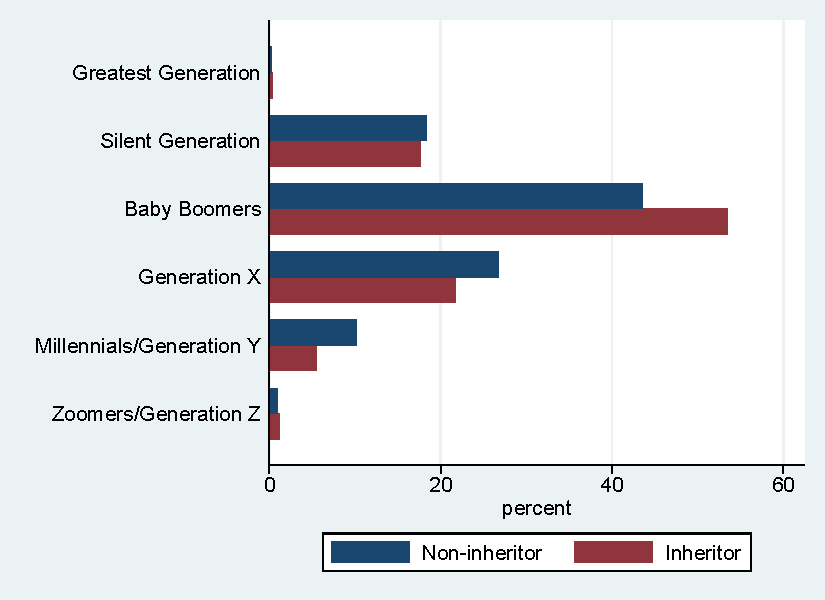
\includegraphics[width=0.7\textwidth]{Figures/Inheritors/birthcohort_inh.pdf}
    \caption{Birth Cohort Distribution of Inheritors}
    \label{fig:inheritor_cohorts}
    \caption*{Source: Author's calculations on SHIW 2022 data.}
\end{figure}

This age gap directly translates to differences in employment status (Figure \ref{fig:inheritor_workstatus}). The single largest category for inheritors is "Retired" (nearly 50\%), a significantly higher proportion than for non-inheritors (around 42\%). Conversely, non-inheritors are more likely to be in active employment categories such as "Worker" or "Clerk."

\begin{figure}[ht!]
    \centering
    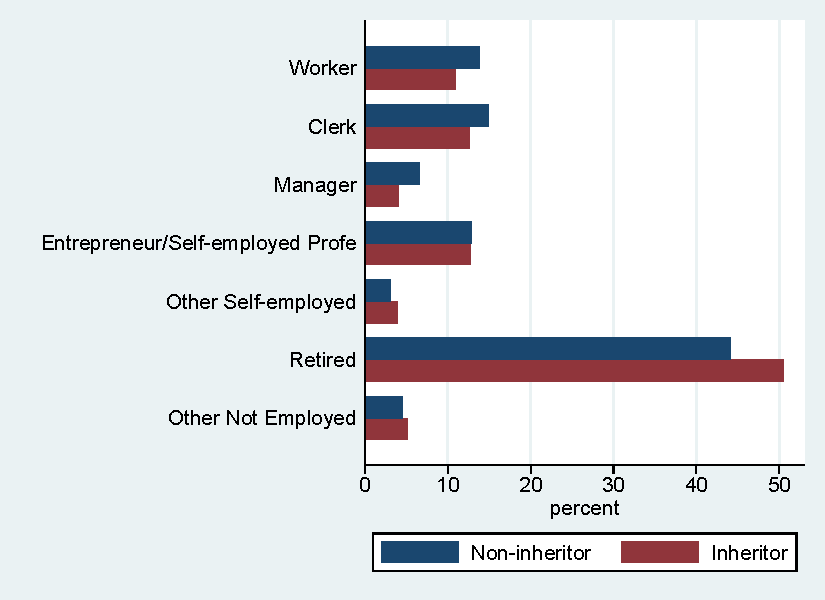
\includegraphics[width=0.7\textwidth]{Figures/Inheritors/workstatus_inh.pdf}
    \caption{Working Status of Inheritors}
    \label{fig:inheritor_workstatus}
    \caption*{Source: Author's calculations on SHIW 2022 data.}
\end{figure}

An analysis of educational attainment reveals a significant story of intergenerational upward mobility across the entire population. Figure \ref{fig:inheritor_parent_edu} shows that the parents of \textit{both} inheritors and non-inheritors predominantly had low levels of formal education, with a majority holding at most a primary school diploma. This reflects the educational norms of their time and suggests their wealth was likely accumulated through work and saving during Italy's post-war economic expansion.

In stark contrast, Figure \ref{fig:inheritor_edu} shows that the children's generation is far more educated. However, what is most striking is the similarity between the two groups: the educational distribution of inheritors is almost identical to that of non-inheritors. This suggests that while one generation built a foundation of material wealth, the subsequent increase in educational attainment was a widespread societal phenomenon, not a feature unique to those who would later inherit property.

\begin{figure}[ht!]
    \centering
    \begin{subfigure}[b]{0.48\textwidth}
        \centering
        \includegraphics[width=\textwidth]{Figures/Inheritors/parentedu_inh.pdf}
        \caption{Parental Education Level}
        \label{fig:inheritor_parent_edu}
    \end{subfigure}
    \hfill
    \begin{subfigure}[b]{0.48\textwidth}
        \centering
        \includegraphics[width=\textwidth]{Figures/Inheritors/education_inh.pdf}
        \caption{Own Education Level}
        \label{fig:inheritor_edu}
    \end{subfigure}
    \caption{Educational Attainment of Inheritors and Their Parents}
    \label{fig:inheritor_education_comparison}
    \caption*{Source: Author's calculations on SHIW 2022 data.}
\end{figure}

Finally, the geographical distribution of the two groups by birth area, presented in Figure \ref{fig:inheritor_geo}, is also remarkably similar. For both inheritors and non-inheritors, the highest concentration is in the South of Italy, followed by the North, and then the Centre. This reinforces that real estate inheritance is not confined to a specific region but is a widespread national phenomenon. Unsurprisingly, those born outside of Italy ("Foreign") make up a very small fraction of both groups and a negligible share of inheritors, underscoring that this form of wealth transfer is closely tied to multi-generational presence within the nation.

\begin{figure}[ht!]
    \centering
    \includegraphics[width=0.7\textwidth]{Figures/Inheritors/birtharea_inh.pdf}
    \caption{Geographical Area of Birth of Inheritors}
    \label{fig:inheritor_geo}
    \caption*{Source: Author's calculations on SHIW 2022 data.}
\end{figure}

%%%%%%%%%%%%%%%%%%%%% SUBSECTION 4.3.2 %%%%%%%%%%%%%%%%%%%%
\subsection{Distribution of Income and Wealth within Inheritors}
\label{sec:4.3.2}

This section examines the level of inequality \textbf{within} the inheritor subsample and compares it to that of the general population analyzed in Section \ref{sec:4.1.1}. This comparison helps to understand whether the group of inheritors is more or less homogeneous than the population as a whole.

Table \ref{tab:ineqindexes_inh} presents the inequality indices calculated only for the 1,307 inheritor households. The results are revealing. For both income and wealth, the Gini coefficient is lower for the inheritor subsample (0.339 for income and 0.622 for wealth) than for the entire population (0.365 and 0.659, respectively). This indicates that inheritors are, as a group, more economically equal than the general population (\ref{tab:ineqindexes})

\begin{table}[htbp]\centering
\caption{Inequality Indices for Income and Wealth}
\begin{tabular}{l*{3}{c}}
\toprule
                    &           D&            &            \\
                    &  Net Income&  Net Wealth&Transformed Net Wealth\\
\midrule
Gini Coefficient    &    .3394925&    .6224657&    .6224299\\
p90/p10 Ratio       &    4.184526&    11.99262&    11.99262\\
p90/p50 Ratio       &    2.036225&    3.125217&    3.125217\\
p10/p50 Ratio       &    .4866083&     .260595&     .260595\\
p75/p25 Ratio       &    2.074891&     3.39715&     3.39715\\
GE(0)               &    .2028861&           .&    .7268937\\
GE(1)               &    .2229152&           .&    1.039035\\
GE(2)               &    .3777336&    6.143388&    6.143094\\
Atk(0.5)            &     .099259&           .&    .3454145\\
Atk(1)              &    .1836288&           .&    .5165917\\
Atk(2)              &    .3483267&           .&    .9962659\\
\bottomrule
\end{tabular}
\end{table}


The difference is particularly stark when looking at the percentile ratios for wealth. While the p90/p10 ratio for the entire population was over 247, within the inheritor group it is dramatically smaller at approximately 12. This is because the "poorest" inheritors are still homeowners with significant housing equity, which places them far above the asset-poor households that occupy the bottom of the overall wealth distribution.

The Lorenz curves presented in Figure \ref{fig:lorenz_curves_inh} provide a visual confirmation of this finding. Both the income and wealth curves for the inheritor subsample lie slightly closer to the 45-degree line of perfect equality than their counterparts for the general population (see Figure \ref{fig:lorenz_curves}). This visually demonstrates the lower Gini coefficients and the more compressed distribution of resources within this group. A formal test for Lorenz dominance confirms that the net income Lorenz curve dominates the net wealth curve for inheritors, with the results available in Appendix \ref{appendix:A} (Table \ref{tab:lorenz_contrast_inheritors}).

\begin{figure}[ht!]
    \centering
    \includegraphics[width=0.8\textwidth]{Figures/Inheritors/lorenz_curves.pdf}
    \caption{Lorenz Curves for Net Income and Net Wealth (Inheritor Subsample)}
    \label{fig:lorenz_curves_inh}
    \caption*{Source: Author's calculations on SHIW 2022 data. The shaded area represents the 95\% confidence interval.}
\end{figure}

In conclusion, inheritors are more homogeneous (at least from the point of view of net wealth) than the whole population. Inheritance appears to lift households to a relatively high and uniform floor of wealth, reducing the extreme disparities observed across the population as a whole.

%%%%%%%%%%%%%%%%%%%%% SUBSECTION 4.3.3 %%%%%%%%%%%%%%%%%%%%
\subsection{The Nature and Significance of Inherited Real Estate}
\label{sec:4.3.3}

Having profiled the inheritor household, this final section examines the inherited asset itself. The analysis focuses first on the distribution of the market value of these properties and then on their significance as a component of the household's total net wealth.

The 2022 market value of inherited homes is, much like overall wealth, highly right-skewed. Table \ref{tab:2022mktvalue} details this distribution. While the median value is a substantial €150,000, the mean is significantly higher at over €201,800, confirming a long tail of very valuable properties. The distribution covers a wide range: while the bottom 10\% of inherited properties are valued at €50,000 or less, the top 1\% are worth €1,000,000 or more.

Table \ref{tab:ineq_value2022} quantifies the inequality within the distribution of these inherited assets. The Gini coefficient stands at 0.443. While high, this is considerably lower than the Gini for overall net wealth (0.659), which suggests that the value of inherited homes is more evenly distributed than total wealth. The p90/p10 ratio of 7 confirms this; the top is much closer to the bottom compared to the explosive ratios seen for total wealth.

\input{Tables/Inheritors/value2022_distr_ineq}

To better visualize this skewed distribution, Figure \ref{fig:log_value_inher_home} presents a histogram of the log-transformed values. The plot reveals a roughly normal distribution centered around the value of a typical family home, but with a clear right tail representing the high-value estates identified in the percentile data.

\begin{figure}[ht!]
    \centering
    \includegraphics[width=0.7\textwidth]{Figures/Inheritors/log_2022mktvalue.pdf}
    \caption{Distribution of the Log-Transformed Value of Inherited Homes (2022) with a Normal Distribution overlay}
    \label{fig:log_value_inher_home}
    \caption*{Source: Author's calculations on SHIW 2022 data.}
\end{figure}


To understand the economic impact of these transfers, we now turn to the "inheritance share," defined as the ratio of the inherited home's value to the household's total net wealth. This measure reveals how central the inheritance is to the family's balance sheet. The analysis is performed from two perspectives, with detailed tables available in Appendix \ref{appendix:A} (Tables \ref{tab:inh_share_pop} - \ref{tab:inh_share_inh}).

The analysis is performed from two perspectives, as shown in Figure \ref{fig:inheritance_share_analysis}. First, a micro-level view examines the share's importance \textbf{within the subsample of inheritors} (Figure \ref{fig:share_within_inheritors}). The results are striking: for the least wealthy inheritors (the bottom deciles), the inherited home constitutes nearly their entire net worth, with the share often exceeding 90\%. For the wealthiest inheritors, while the absolute value of the home is high, its share of their total wealth is smaller, as they also possess significant financial and other assets. This shows that for many, the inherited home is not just an asset, but the primary foundation of their economic security.


\begin{figure}[ht!]
    \centering
    \begin{subfigure}[b]{0.48\textwidth}
        \centering
        \includegraphics[width=\textwidth]{Figures/Inheritors/inhshare_inheritors.pdf}
        \caption{Share Within Inheritor Wealth Deciles}
        \label{fig:share_within_inheritors}
    \end{subfigure}
    \hfill
    \begin{subfigure}[b]{0.48\textwidth}
        \centering
        \includegraphics[width=\textwidth]{Figures/Inheritors/inhshare_pop.pdf}
        \caption{Share Within Overall Wealth Deciles}
        \label{fig:share_overall_population}
    \end{subfigure}
    \caption{Average Inheritance Share by Wealth Deciles}
    \label{fig:inheritance_share_analysis}
    \caption*{Source: Author's calculations on SHIW 2022 data.}
\end{figure}

Second, a macro-level view assesses the role of inherited real estate in shaping the \textbf{overall wealth distribution} (Figure \ref{fig:share_overall_population}). The pattern is similar: inherited wealth constitutes a larger share of total wealth for the lower-middle deciles of the general population compared to the top deciles. This reinforces the finding from Section \ref{sec:4.1.2} that inheritance acts as a "wealth floor," having its most significant relative impact on households that would otherwise have fewer assets.

%This concludes the descriptive analysis. The evidence clearly shows that inherited real estate is a significant asset, particularly for less wealthy recipients, and that its distribution, while unequal, is less concentrated than that of overall wealth.

%%%%%%%%%%%%%%%%%%%%%%%%%%%%% SECTION 4.4 %%%%%%%%%%%%%%%%%%%%%%%%%%%%%%%%%%%%%%%%%%%%%%%%%%%%%
\section{Bivariate Correlation Analysis}\label{sec:4.4}
Having detailed the distributions of wealth and the characteristics of different household groups, the analysis now moves to formally test the unconditional relationships between inheritance status and key socio-economic variables. This section uses bivariate tests to identify which household characteristics are statistically associated with the probability of having inherited a home, providing a preliminary look at the correlates of real estate inheritance.

A methodological note is warranted. To correctly account for the complex survey design of the SHIW, standard t-tests and chi-squared tests are not appropriate. Therefore, for continuous variables, the difference in means is assessed by regressing the variable on a binary indicator for inheritance status using the \texttt{svy: regress} command in Stata. The coefficient on the inheritor dummy represents the average difference between the two groups, and its t-statistic provides a test of significance. For categorical variables, the association is tested using the \textit{Rao-Scott corrected F-statistic}, which is the appropriate design-adjusted equivalent of the Pearson chi-squared test (\cite{RaoScott}).

%%%%%%%%%%%%%%%%%%%%%%% SUBSECTION 4.4.1 %%%%%%%%%%%%%%%%%%%%%%%%%%%%%%%%%%%%%%%
\subsection*{The Full Sample: Inheritors vs. Non-Inheritors}\label{sec:4.4.1}
The first analysis compares inheritors to all other households in the sample, a group that includes both renters and "self-made" owners. Table \ref{tab:bivariate_cont_full} presents the results for the continuous variables.

The results show several significant unconditional differences. Inheritor households tend to be smaller, have substantially higher net wealth (on average, €142,782 more), and a much higher saving rate. Interestingly, there is no statistically significant difference in their average net income or the market value of their residence when compared to the entire non-inheritor group.

\begin{tabular}{l*{5}{c}}
\toprule
                    & reg\_results&            &            &            &            \\
                    &     Model\_F&     Model\_p&Coef\_Inheritor& t-statistic&     p-value\\
\midrule
 $\times$ of Household Components&     22.5553&    3.11e-06&   -.2945772&   -4.749242&    3.11e-06\\
Net Income          &    2.118853&    .1464977&   -1855.213&   -1.455628&    .1464977\\
Net Wealth          &    5.792103&    .0166773&      142782&    2.406679&    .0166773\\
Saving Rate         &    23.85678&    1.66e-06&     232.622&    4.884341&    1.66e-06\\
Residence Market Value (at 2022)&    .8923688&    .3455648&    9990.787&    .9446527&    .3455648\\
\bottomrule
\end{tabular}


Table \ref{tab:bivariate_cat_full} presents the results of the association tests for the categorical variables. Here, the associations are very strong. There is a highly significant relationship between being an inheritor and the household head's birth cohort, birth area, parental education, and a quite strong relationship with the working status. The only characteristic that shows no significant association is the head's own education level (p-value of 0.361).

\begin{tabular}{l*{4}{c}}
\toprule
                    &     results&            &            &            \\
                    & F-statistic&         df1&         df2&     p-value\\
\midrule
Birth cohort        &    8.743296&     4.27899&    1339.324&    2.64e-07\\
Birth Area          &    8.180981&    2.321223&    726.5429&    .0001328\\
Education           &     1.09867&    5.857781&    1833.486&    .3605484\\
Parental Education  &    5.541883&    4.974245&    1556.939&    .0000475\\
Working Status      &    2.402893&    5.108172&    1598.858&    .0338949\\
\bottomrule
\end{tabular}


%%%%%%%%%%%%%%%%%%%%%%% SUBSECTION 4.4.2 %%%%%%%%%%%%%%%%%%%%%%%%%%%%%%%%%%%%%%%
\subsection*{The Homeowner Subsample: Inheritor-Owners vs. "Self-Made" Owners}\label{sec:4.4.2}

The analysis is now restricted to the 7,654 homeowners to compare those who inherited their home against those who acquired it through other means. This comparison is more direct, as it removes the confounding effect of renters.

The results in Table \ref{tab:bivariate_cont_owners} are markedly different from the full sample analysis. Within the homeowner group, inheritors have significantly lower average net income than their "self-made" counterparts. This aligns with the descriptive finding that purchasing a home often requires a higher concurrent income stream. Furthermore, the large wealth gap observed previously disappears; there is no statistically significant difference in the average net wealth or residence value between the two types of owners. This suggests that while inheritance is a key pathway to home-ownership, "self-made" owners eventually catch up in terms of total wealth.

\begin{tabular}{l*{5}{c}}
\toprule
                    &reg\_results2&            &            &            &            \\
                    &     Model\_F&     Model\_p&Coef\_Inheritor& t-statistic&     p-value\\
\midrule
 $\times$ of Household Components&    31.47185&    4.45e-08&    -.347533&   -5.609977&    4.45e-08\\
Net Income          &    32.94756&    2.24e-08&    -8028.47&   -5.739997&    2.24e-08\\
Net Wealth          &    .4054071&    .5247753&    40321.08&    .6367159&    .5247753\\
Saving Rate         &    3.246971&    .0725177&   -.0351918&   -1.801935&    .0725177\\
Residence Market Value (at 2022)&    1.933374&    .1653776&   -16319.58&   -1.390458&    .1653776\\
\bottomrule
\end{tabular}


The associations among categorical variables also shift (Table \ref{tab:bivariate_cat_owners}). Parental education remains a very strong correlate, as does birth cohort. However, the association with birth area is no longer significant. Interestingly, both the household head's own education and working status are now marginally significant. These bivariate results highlight several strong correlations, but also reveal that these relationships can change depending on the sample definition, which would have motivated a multivariate analysis to disentangle these effects.

\begin{tabular}{l*{4}{c}}
\toprule
                    &    results2&            &            &            \\
                    & F-statistic&         df1&         df2&     p-value\\
\midrule
Birth cohort        &    3.494021&    4.296521&    1344.811&    .0061835\\
Birth Area          &    1.528118&    2.440385&    763.8406&    .2129537\\
Education           &    2.038918&    5.899299&    1846.481&    .0586968\\
Parental Education  &    6.484309&    4.988496&    1561.399&    5.74e-06\\
Working Status      &    2.091389&    5.299621&    1658.781&     .059804\\
\bottomrule
\end{tabular}



%%%%%%%%%%%%%%%%%%%%%%%%%%%%%%%%%%%%%%%%%%%%%%%%%%%%%%%%%%%%%%%%%%%%%%%%%%%%%%% CHAPTER 5 %%%%%%%%%%%%%%%%%%%%%%%%%%%%%%%%%%%%%%%%%%%%%%%%%%%%%%%%%%%%%%%%%%%%%%%%%%%%%%%%%%%%
%\chapter{The Correlates of Real Estate Inheritance: An Econometrical Analysis}
%\label{ch:5}

%This chapter moves from descriptive to inferential analysis to identify the key socio-economic factors associated with receiving a real estate inheritance in Italy. The analysis begins with a preliminary examination of the bivariate relationships between inheritance status and a range of household characteristics. This initial step helps to identify unconditional correlations and motivates the subsequent multivariate analysis. The core of the chapter then involves specifying and estimating three different binary choice models—Linear Probability, Probit, and Logit—to robustly model the probability of being an inheritor. The results will be presented in the form of marginal effects to ensure comparability across models, followed by a discussion of the most significant and consistent findings.

%%%%%%%%%%%%%%%%%%%%% SECTION 5.1 %%%%%%%%%%%%%%%%%%%%%%%%%%
%\section{Bivariate Analysis}
%\label{sec:5.1}

%Before proceeding to the multivariate regression models, this section explores the simple bivariate relationships between the key variables of interest. This preliminary step aims to identify which household characteristics are unconditionally associated with the probability of having inherited a home. The analysis is conducted first on the full sample of households and then on the restricted subsample of homeowners to draw out any differences.

%A methodological note is warranted. To correctly account for the complex survey design of the SHIW, standard t-tests and chi-squared tests are not appropriate. Therefore, for continuous variables, the difference in means is assessed by regressing the variable on a binary indicator for inheritance status using the \texttt{svy: regress} command in Stata. The coefficient on the inheritor dummy represents the average difference between the two groups, and its t-statistic provides a test of significance. For categorical variables, the association is tested using the \textit{Rao-Scott corrected F-statistic}, which is the appropriate design-adjusted equivalent of the Pearson chi-squared test (\cite{RaoScott}).


%%%%%%%%%%%%%%%%%% SUBSECTION 5.1.1 %%%%%%%%%%%%%%%%%%%%%%%%
%\subsection{The Full Sample: Inheritors vs. Non-Inheritors} \label{subsec:5.1.1}

%The first analysis compares inheritors to all other households in the sample, including renters and "self-made" owners. Table \ref{tab:bivariate_cont_full} presents the results for the continuous variables.

%\begin{tabular}{l*{5}{c}}
\toprule
                    & reg\_results&            &            &            &            \\
                    &     Model\_F&     Model\_p&Coef\_Inheritor& t-statistic&     p-value\\
\midrule
 $\times$ of Household Components&     22.5553&    3.11e-06&   -.2945772&   -4.749242&    3.11e-06\\
Net Income          &    2.118853&    .1464977&   -1855.213&   -1.455628&    .1464977\\
Net Wealth          &    5.792103&    .0166773&      142782&    2.406679&    .0166773\\
Saving Rate         &    23.85678&    1.66e-06&     232.622&    4.884341&    1.66e-06\\
Residence Market Value (at 2022)&    .8923688&    .3455648&    9990.787&    .9446527&    .3455648\\
\bottomrule
\end{tabular}


%The results show several significant unconditional differences. Inheritor households tend to be smaller, have substantially higher net wealth (on average, €142,782 more), and a much higher saving rate. Interestingly, there is no statistically significant difference in their average net income or the market value of their residence when compared to the entire non-inheritor group.

%Table \ref{tab:bivariate_cat_full} presents the results of the association tests for the categorical variables.

%\begin{tabular}{l*{4}{c}}
\toprule
                    &     results&            &            &            \\
                    & F-statistic&         df1&         df2&     p-value\\
\midrule
Birth cohort        &    8.743296&     4.27899&    1339.324&    2.64e-07\\
Birth Area          &    8.180981&    2.321223&    726.5429&    .0001328\\
Education           &     1.09867&    5.857781&    1833.486&    .3605484\\
Parental Education  &    5.541883&    4.974245&    1556.939&    .0000475\\
Working Status      &    2.402893&    5.108172&    1598.858&    .0338949\\
\bottomrule
\end{tabular}


%Here, the associations are very strong. There is a highly significant relationship between being an inheritor and the household head's birth cohort, birth area, parental education, and working status. The only characteristic that shows no significant association is the head's own education level (p-value of 0.361), a surprising finding that will be explored further in the multivariate context.


%%%%%%%%%%%%%%%%%% SUBSECTION 5.1.2 %%%%%%%%%%%%%%%%%%%%%%%%
%\subsection{The Homeowner Subsample: Inheritor-Owners vs. "Self-Made" Owners} \label{subsec:5.1.2}

%The analysis is now restricted to the 7,654 homeowners to compare those who inherited their home against those who acquired it through other means. This comparison is more direct, as it removes the confounding effect of renters.

%\begin{tabular}{l*{5}{c}}
\toprule
                    &reg\_results2&            &            &            &            \\
                    &     Model\_F&     Model\_p&Coef\_Inheritor& t-statistic&     p-value\\
\midrule
 $\times$ of Household Components&    31.47185&    4.45e-08&    -.347533&   -5.609977&    4.45e-08\\
Net Income          &    32.94756&    2.24e-08&    -8028.47&   -5.739997&    2.24e-08\\
Net Wealth          &    .4054071&    .5247753&    40321.08&    .6367159&    .5247753\\
Saving Rate         &    3.246971&    .0725177&   -.0351918&   -1.801935&    .0725177\\
Residence Market Value (at 2022)&    1.933374&    .1653776&   -16319.58&   -1.390458&    .1653776\\
\bottomrule
\end{tabular}


%The results in Table \ref{tab:bivariate_cont_owners} are markedly different from the full sample analysis. Within the homeowner group, inheritors have significantly \textbf{lower average net income} than their "self-made" counterparts. This aligns with the descriptive finding that purchasing a home often requires a higher concurrent income stream. Furthermore, the large wealth gap observed previously disappears; there is no statistically significant difference in the average net wealth or residence value between the two types of owners. This suggests that while inheritance is a key pathway to homeownership, "self-made" owners eventually catch up in terms of total wealth.

%\begin{tabular}{l*{4}{c}}
\toprule
                    &    results2&            &            &            \\
                    & F-statistic&         df1&         df2&     p-value\\
\midrule
Birth cohort        &    3.494021&    4.296521&    1344.811&    .0061835\\
Birth Area          &    1.528118&    2.440385&    763.8406&    .2129537\\
Education           &    2.038918&    5.899299&    1846.481&    .0586968\\
Parental Education  &    6.484309&    4.988496&    1561.399&    5.74e-06\\
Working Status      &    2.091389&    5.299621&    1658.781&     .059804\\
\bottomrule
\end{tabular}


%The associations among categorical variables also shift (Table \ref{tab:bivariate_cat_owners}). Parental education remains a very strong correlate, as does birth cohort. However, the association with birth area is no longer significant. Interestingly, both the household head's own education and working status are now marginally significant.

%These bivariate results highlight several strong correlations, but also reveal that these relationships can change depending on the sample definition. This underscores the need for a multivariate regression analysis to disentangle these effects, which is the subject of the next section.


%%%%%%%%%%%%%%%%%%%%% SECTION 5.2 %%%%%%%%%%%%%%%%%%%%%%%%%%
%\section{Model Specification and Variables}\label{sec:5.2}

%Building on the bivariate analysis, this section specifies the full multivariate models to be estimated. The theoretical underpinnings of the Linear Probability, Probit, and Logit models were detailed in Section \ref{sec:3.4}. Here, the focus is on defining the specific dependent and independent variables used in the estimation and outlining the hypotheses regarding their expected effects.

%%\subsection*{Dependent Variables}
%The analysis employs two distinct binary dependent variables to address the two central research questions:
%\begin{enumerate}
    %\item \textbf{Inheritor}: A binary variable equal to 1 for households that acquired their main residence through full inheritance, and 0 for all other households. This is the dependent variable for the models estimated on the full sample.
    %\item \textbf{Inheritor-Owner}: A binary variable defined only for the subsample of homeowners, equal to 1 for households that inherited their home and 0 for those who acquired it through other means. This is the dependent variable for the models estimated on the homeowner subsample (7,654 households).
%\end{enumerate}

%\subsection*{Independent Variables and Hypothesized Effects}
%The selection of independent variables is guided by the economic literature on intergenerational transfers and wealth accumulation, as well as the findings from the descriptive analysis in Chapter \ref{ch:4}. The full model includes a range of socio-demographic and economic characteristics intended to capture the key factors correlated with the probability of receiving a real estate inheritance. Table \ref{tab:variable_hypotheses} lists these variables and their hypothesized effect on the probability of being an inheritor.

%\begin{landscape}
%\begin{table}[ht!]
%\centering
%\caption{Independent Variables and Hypothesized Effects}
%\label{tab:variable_hypotheses}
%\begin{tabular}{lp{8cm}c}
%\hline\hline
%Variable & Description & Expected Sign \\
%\hline
%\textit{Intergenerational Factors} & & \\
%Parental Education & Highest education level of either parent (categorical). & + \\
%Birth Cohort & Generational cohort of the household head (categorical). & +/- \\
%Birth Area & Geographical area of birth (categorical). & +/- \\
%\hline
%\textit{Household Characteristics} & & \\
%Education & Education level of the household head (categorical). & + \\
%Working Status & Employment status of the household head (categorical). & +/- \\
%Household Size & Number of components in the household. & - \\
%\hline
%\textit{Economic Resources} & & \\
%Log Net Income & Natural log of household net disposable income. & + \\
%Asinh Net Wealth & Inverse hyperbolic sine of household net wealth. & + \\
%Saving Rate & Ratio of household savings to net income. & + \\
%\hline\hline
%\end{tabular}
%\vspace{0.5em}
%\caption*{The expected sign indicates the hypothesized direction of the relationship with the probability of being an inheritor.}
%\end{table}
%\end{landscape}

%The hypotheses are grounded in established theory. A positive sign is expected for \textbf{Parental Education}, as it serves as a strong proxy for the socio-economic status of the previous generation. The effect of \textbf{Birth Cohort} is expected to be non-linear, capturing the life-cycle effect where the probability of having inherited is highest for older generations. The household's own \textbf{Education}, \textbf{Net Income}, \textbf{Net Wealth}, and \textbf{Saving Rate} are all expected to be positively correlated with inheritance, as these factors are associated with greater economic resources and opportunity. Conversely, a larger \textbf{Household Size} may be negatively associated with the probability of residing in an inherited home, potentially due to space constraints. The effects of \textbf{Birth Area} and \textbf{Working Status} are ambiguous a priori and are included as important controls.

%%%%%%%%%%%%%%%%%%%%% SECTION 5.3 %%%%%%%%%%%%%%%%%%%%%%%%%%
%\section{Estimation Results}\label{sec:5.3}

%%%%%%%%%%%%%%%%%%%%% SECTION 5.4 %%%%%%%%%%%%%%%%%%%%%%%%%%
%\section{Discussion of the Key Findings}\label{sec:5.4}

%\section{Robustness Checks}
%...


%%%%%%%%%%%%%%%%%%%%%%%%%%%%%%%%%%%%%%%%%%%%%%%%%%%%%%%%%%%%%%%%%%%%%%%%%%%%%%% CHAPTER 5 %%%%%%%%%%%%%%%%%%%%%%%%%%%%%%%%%%%%%%%%%%%%%%%%%%%%%%%%%%%%%%%%%%%%%%%%%%%%%%
\chapter{Microsimulation of Inheritance Tax Reform} \label{ch:5}

Having analyzed the characteristics of inheritor households and the factors correlated with receiving a real estate inheritance, this chapter moves from description to policy evaluation. It employs the static microsimulation model detailed in Section \ref{sec:3.4} to quantify the potential first-order redistributive impact of replacing Italy's current inheritance tax system with a range of international alternatives. To establish a benchmark for the analysis, Section \ref{sec:5.1} begins by outlining the current Italian inheritance tax regime, while Section \ref{sec:5.2} recaps the pre-reform baseline level of wealth inequality. The core of the analysis is presented in Section \ref{sec:5.3}, which simulates a series of international tax regimes—grouped into flat-rate and progressive-rate systems—and calculates the additional revenue and redistributive transfers generated by each. Following this, Section \ref{sec:5.4} provides a comprehensive summary and comparative analysis of all simulation outcomes. The chapter concludes with Section \ref{sec:5.5}, which discusses the key findings and their policy implications for tackling wealth inequality in Italy.

%%%%%%%%%%%%%%%%%%%% SECTION 5.1 %%%%%%%%%%%%%%%%%%%%%%%
\section{The Current Inheritance Tax System in Italy} \label{sec:5.1}

The Italian inheritance and gift tax system, governed by Decree Law No. 262 of 2006 (\cite{decretoleggeitalia}), is characterized by a structure of rates and allowances that vary significantly based on the relationship between the deceased and the beneficiary. The system is defined by four main categories:

\begin{itemize}
    \item A rate of \textbf{4\%} on the value exceeding a \textbf{€1 million} allowance for each beneficiary, applicable to transfers between spouses and direct-line relatives (ascendants and descendants).
    \item A rate of \textbf{6\%} on the value exceeding a \textbf{€100,000} allowance for transfers between siblings.
    \item A rate of \textbf{6\%} on the total value transferred, with no allowance, for other relatives up to the fourth degree and relatives-in-law up to the third degree.
    \item A rate of \textbf{8\%} on the total value transferred, with no allowance, for all other individuals.
\end{itemize}
An additional allowance of €1.5 million is provided for beneficiaries with a recognized severe disability.

As discussed in the methodological limitations (Section \ref{sec: 3.5.2}), the SHIW dataset does not contain information on the specific relationship between the heir and the deceased. Consequently, for the purpose of this microsimulation, a simplifying assumption has been made: all inheritances are modeled as vertical transfers from a parent to a child. This means that the baseline Italian tax liability for all households in the simulation is calculated using the first and most favorable regime: a \textbf{4\% flat tax on the value of the inherited property exceeding the €1 million threshold}.

This high threshold makes the Italian system one of the most lenient among advanced economies. Its practical effect is that a vast majority of inheritances are completely exempt from taxation. Applying this rule to the inheritor households in the 2022 SHIW sample reveals the very narrow scope of the current tax base.

\vspace{1em}
\noindent\fbox{%
    \parbox{\dimexpr\textwidth-2\fboxsep-2\fboxrule\relax}) would be liable for any inheritance tax.
        
        A sensitivity analysis using a more varied, hypothetical distribution of heir types (80\% parent-child, 15\% siblings, 5\% other relatives) reveals a much broader tax base. In this scenario, the number of taxpayers would be composed of approximately 23,000 parent-child heirs, 442,000 siblings, and 196,000 other relatives. 
        
        This results in a total of approximately \textbf{661,000} tax-paying households, meaning the share of inheritance events triggering a tax payment rises dramatically to \textbf{17.0\%}.
    }%
}
\vspace{1em}

This low number of taxpayers serves as the starting point for the subsequent policy simulations, which explore how alternative tax structures could broaden the tax base and generate revenue for redistribution.


%%%%%%%%%%%%%%%%%%%% SECTION 5.2 %%%%%%%%%%%%%%%%%%%%%%%
\section{The Baseline Scenario: Pre-Reform Wealth Inequality}\label{sec:5.2}

Before evaluating the impact of potential policy reforms, it is essential to establish a clear baseline measure of wealth inequality in Italy. This baseline serves as the benchmark against which the redistributive effects of all subsequent simulations will be measured. The pre-reform scenario is based on the distribution of household net wealth in 2022, as captured by the SHIW data.

A detailed descriptive analysis of this distribution, including a decomposition by inheritance status, was presented in Subsections \ref{sec:4.1.1} and \ref{sec:4.1.3}. As established in that chapter, wealth in Italy is highly concentrated. The overall Gini coefficient for household net wealth stands at \textbf{0.659}, indicating a profound level of inequality.

Table \ref{tab:baseline_inequality} summarizes the key features of this pre-reform landscape, recapping the main findings from the decomposition analysis (more details can be found in Tables \ref{tab:ineqindexes} and \ref{tab:decompositioninequality}). It highlights not only the high overall inequality but also the significant disparities both within and between the groups of inheritors and non-inheritors.

\begin{table}[ht!]
\centering
\caption{Baseline Wealth Inequality Scenario (2022)}
\label{tab:baseline_inequality}
\begin{tabular}{lc}
\toprule
\textbf{Indicator} & \textbf{Value} \\
\midrule
\multicolumn{2}{l}{\textit{Overall Population}} \\
\quad Gini Coefficient & 0.6593 \\
\midrule
\multicolumn{2}{l}{\textit{Subgroup Inequality (Within-Group Gini)}} \\
\quad Non-Inheritors & 0.6641 \\
\quad Inheritors & 0.6225 \\
\midrule
\multicolumn{2}{l}{\textit{Between-Group Disparity (Relative Mean Wealth)}} \\
\quad Non-Inheritors & 0.927 \\
\quad Inheritors & 1.410 \\
\bottomrule
\end{tabular}
\vspace{0.5em}
\caption*{Source: Author's calculations on SHIW 2022 data.}
\end{table}

The baseline scenario is thus defined by three key characteristics: a high overall level of wealth concentration; a substantial economic advantage for inheritor households, who on average possess over 40\% more wealth than the typical household; and the fact that the vast majority of this inequality arises from disparities \textit{within} each of the two groups. This detailed picture of the pre-reform distribution provides the necessary starting point for assessing the potential of different tax systems to alter these outcomes.


%%%%%%%%%%%%%%%%%%%% SECTION 5.3 %%%%%%%%%%%%%%%%%%%%%%
\section[Policy Scenarios: Simulating International Tax Regimes]{Policy Scenarios: Simulating International\\ Tax Regimes} \label{sec:5.3}

With the baseline scenario established, the analysis now turns to the core exercise of this thesis. This process is modeled in two distinct stages: first, the generation of revenue through the application of a new tax law, and second, the redistribution of that revenue. This section addresses the first stage by simulating the replacement of the current Italian inheritance tax with systems modeled on those of various other countries.

The goal is to quantify two key metrics: the potential additional revenue each system could generate, and the immediate, first-order impact of these tax payments on wealth inequality. To isolate this latter effect, we calculate an \textbf{intermediate Gini coefficient}. This measure reflects a counterfactual wealth distribution where the simulated tax liability has been subtracted from inheritor households, but the revenue has \textit{not yet} been distributed. The change from the baseline Gini (0.6593) to this intermediate Gini represents the pure \textbf{tax effect}—that is, the change in inequality caused solely by the collection of the tax itself. The revenue collected and the tax effects for each regime are presented in the subsections below.


%%%%%%%%%%%%%%% SUBSECTION 5.3.1 %%%%%%%%%%%%%%%%%%%%%%
\subsection{Simulating Flat-Rate Regimes}

The first set of policy scenarios involves tax systems whose main feature is the use of a single flat tax rate on the value of an inheritance exceeding a specified allowance. While this approach differs from the progressive-rate structures analyzed later, the complexity of the systems can vary. The Irish regime is a straightforward example, whereas the UK regime, like the Italian one, incorporates significant distinctions based on the heir's relationship to the deceased, albeit primarily through its allowance structure rather than through different tax rates. Two such regimes are simulated: that of Ireland and the United Kingdom.

%%%%%%%%%%%%%%% SUBSUBECTION 5.3.1.1 %%%%%%%%%%%%%%%%%
\subsubsection{The Irish Regime}

The Irish inheritance tax system (Capital Acquisitions Tax) is structured around different tax-free thresholds depending on the relationship to the donor. For transfers from a parent to a child (Group A), the allowance in 2022 was \textbf{€335,000}. The value of any inheritance exceeding this threshold is subject to a flat tax rate of \textbf{33\%} (\cite{irishlaw}). This represents a significantly lower threshold and a much higher tax rate than the Italian system for direct heirs. The simulation of this regime yields a substantial €45.7 billion in additional revenue, as shown in Table \ref{tab:irish_tax_effect}.

\input{Tables/Microsimulation/Stage 1/Flat Regimes/irish}


%%%%%%%%%%%%%%% SUBSUBECTION 5.3.1.2 %%%%%%%%%%%%%%%%%%
\subsubsection{The United Kingdom Regime}

The inheritance tax system in the United Kingdom is also characterized by a substantial tax-free allowance, known as the "nil-rate band," which was set at £325,000 in 2022 (equivalent to approximately €381,127). An additional "residence nil-rate band" of £175,000 (€205,222) is available if the main home is passed to a direct descendant, bringing the total potential allowance to £500,000 (€586,350 in 2022), provided the total estate is valued at less than £2 million. Any portion of the inheritance above the applicable threshold is taxed at a high flat rate of \textbf{40\%} (\cite{UKlaw}).

This structure makes the UK system more generous than the Irish one in terms of its allowance. Consequently, as shown in Table \ref{tab:uk_tax_effect}, it generates less revenue.

\input{Tables/Microsimulation/Stage 1/Flat Regimes/uk}

%%%%%%%%%%%%%%% SUBSECTION 5.3.2 %%%%%%%%%%%%%%%%%%%%%%
\subsection{Simulating Progressive-Rate Regimes}
In contrast to the flat-rate systems, the second and larger group of policy scenarios involves regimes characterized by progressive tax structures. In these systems, the marginal tax rate increases as the value of the inheritance rises, meaning that wealthier heirs not only pay more tax in absolute terms but also face a higher tax rate on the upper portions of their inheritance.

This approach is common across Continental Europe and parts of Asia and is designed to enhance the redistributive power of the tax. The specific design of these systems varies considerably, however, in terms of their allowances, the number and width of their tax brackets, and the steepness of their rate progression. Some systems, like the Spanish one, introduce additional complexity by making the final tax liability dependent on the heir's pre-existing wealth. The following simulations explore this variety, modeling the systems of France, Belgium, Spain, Finland, Japan, South Korea, and Ecuador to assess their differing impacts on revenue generation and inequality reduction.

%%%%%%%%%%%%%%% SUBSUBECTION 5.3.2.1 %%%%%%%%%%%%%%%%%%
\subsubsection{The Belgian Regime}\label{sec:belgianregime}

Belgium's inheritance tax system is complex, with tax laws set at the regional level. This simulation models the regime of the \textbf{Brussels-Capital Region}, which, like many progressive systems, features multiple tax brackets. For direct-line heirs, the first \textbf{€15,000} of the inheritance is exempt from taxation.

A key feature of the Brussels regime is the application of different tax rates depending on the property's use. A set of reduced rates applies if the inherited property was the main residence of the deceased for at least five years prior to their death (\cite{belgianlaw}). As this information is not available in the SHIW dataset (a limitation discussed in Subsection \ref{sec: 3.5.2}), two distinct scenarios are simulated to provide a bounded estimate of the policy's potential impact:
\begin{itemize}
    \item \textbf{Scenario A} assumes all households are eligible for the \textbf{reduced rates}.
    \item \textbf{Scenario B} assumes no households are eligible, and the higher, \textbf{standard rates} are applied to all.
\end{itemize}

\paragraph{Scenario A: Reduced Rates for Main Residence}

This scenario represents the lower bound of the potential tax revenue. The results in Table \ref{tab:bel_a_tax_effect} show that even this more lenient version of the Belgian system generates a substantial €75.8 billion.

\input{Tables/Microsimulation/Stage 1/Progressive Regime/belgiumA}

\paragraph{Scenario B: Standard Rates}

This scenario provides an upper-bound estimate. As detailed in Table \ref{tab:bel_b_tax_effect}, applying the standard rates generates significantly more revenue, increasing the total to nearly €90 billion.

\input{Tables/Microsimulation/Stage 1/Progressive Regime/belgiumB}

A noteworthy, albeit counterintuitive, detail emerges when comparing the tax effects. Despite generating over €14 billion more in revenue, Scenario B produces a smaller direct reduction in the Gini coefficient (-0.12\%) compared to Scenario A (-0.17\%). This suggests that the additional revenue in Scenario B is disproportionately collected from inheritors in the upper-middle of the wealth distribution, who lose their main residence protection under the standard rates. While this approach is highly effective for revenue generation, the distributional incidence of this broader tax base is less progressively targeted at the very top of the wealth spectrum. Consequently, its immediate impact on the overall Gini coefficient is slightly diluted.

%%%%%%%%%%%%%%% SUBSUBECTION 5.3.2.2 %%%%%%%%%%%%%%%%%%
\subsubsection{The Ecuadorian Regime}

The inheritance tax system in Ecuador provides a distinct example of a progressive structure from South America. The system, which uses the U.S. dollar, is defined by a series of eight tax brackets with marginal rates that increase from 0\% to a top rate of 35\%. A unique and highly significant feature of the law is a \textbf{50\% reduction of the final computed tax liability} for direct-line heirs, a provision that applies to all inheritors in this simulation (\cite{ecuadorianlaw}). This final step substantially lessens the burden of what is otherwise a steeply progressive tax.

As shown in Table \ref{tab:ecu_tax_effect}, the system generates €32.0 billion in additional revenue, an amount comparable to the UK flat-rate system.
\input{Tables/Microsimulation/Stage 1/Progressive Regime/ecuador.tex}

%%%%%%%%%%%%%%% SUBSUBECTION 5.3.2.3 %%%%%%%%%%%%%%%%%%
\subsubsection{The Finnish Regime}

The inheritance tax system in Finland applies a moderate allowance and a clear bracket-based tax calculation. For direct descendants (Category I heirs), the system provides a tax-free allowance for the first \textbf{€19,999} of the inheritance.

The value exceeding this threshold is taxed according to a progressive structure. This structure is defined by a lump-sum tax amount for reaching a given bracket, plus a marginal tax rate applied only to the portion of the value that falls within that bracket. The marginal rates for children range from 7\% for the lowest bracket to a top rate of \textbf{19\%} for inheritances valued at €1 million or more (\cite{finnishlaw}).

\input{Tables/Microsimulation/Stage 1/Progressive Regime/finland}

The regime's relatively low allowance brings a very broad base of inheritances into the tax system, resulting in the collection of a substantial €80.8 billion in additional revenue (Table \ref{tab:fin_tax_effect}). 

Notably, the direct tax effect is a slight increase in the Gini coefficient (+0.04\%). This is because the very low allowance taxes a broad swathe of 'upper-middle' inheritors, while the moderate 19\% top rate is not steep enough to proportionally compress the very top of the distribution. This compresses the middle of the inheritor group downwards more than the top, momentarily increasing measured inequality before the highly redistributive potential of the generated revenue is considered.

%%%%%%%%%%%%%%% SUBSUBECTION 5.3.2.4 %%%%%%%%%%%%%%%%%%
\subsubsection{The French Regime}\label{sec:frenchregime}

The French inheritance tax system is a prominent example of a European progressive-rate model. For direct descendants, the system provides a tax-free allowance of \textbf{€100,000}. The value of the inheritance exceeding this amount is then subject to a series of seven marginal tax brackets, with rates climbing from 5\% to a top rate of 45\% for estates valued over €1.8 million.

Similar to the Belgian case, the French system includes a special provision for the main residence. An abatement of \textbf{20\%} on the market value of the property is granted if the home served as the main residence for both the deceased and the heir at the time of death (\cite{frenchlaw}). Given that this information is not available in the SHIW data, the simulation is again performed under two scenarios:
\begin{itemize}
    \item \textbf{Scenario A} assumes all inheritors qualify for the \textbf{20\% main residence abatement}.
    \item \textbf{Scenario B} assumes no inheritors qualify, and the tax is calculated on the full market value.
\end{itemize}

\paragraph{Scenario A: With Main Residence Abatement}
This scenario represents the most generous application of French law. As shown in Table \ref{tab:fra_a_tax_effect}, this version of the regime generates €60.0 billion in additional revenue.

\input{Tables/Microsimulation/Stage 1/Progressive Regime/frenchA}

\paragraph{Scenario B: Without Main Residence Abatement}
This scenario provides an upper-bound estimate. Without the 20\% abatement, the tax base is larger, leading to a sharp increase in revenue to €90.4 billion (Table \ref{tab:fra_b_tax_effect}).

\input{Tables/Microsimulation/Stage 1/Progressive Regime/frenchB}

%%%%%%%%%%%%%%% SUBSUBECTION 5.3.2.5 %%%%%%%%%%%%%%%%%%
\subsubsection{The Japanese Regime}

The Japanese inheritance tax system is frequently noted for its high top marginal rates, making it one of the most stringent in the world. The system first provides a basic allowance calculated as \textbf{30 million JPY plus 6 million JPY per legal heir}. As the precise number of heirs is unknown, this simulation assumes a single heir for each inheritance, a common household structure among the inheritor sample. This results in a total allowance of 36 million JPY (approximately €260,820 in 2022).

The taxable value exceeding this allowance is then subject to a steeply progressive structure of eight tax brackets (\cite{japaneselaw}). The marginal rates begin at 10\% and rise sharply to a top rate of \textbf{55\%} for the portion of an inheritance valued over 600 million JPY (about €4.35 million).

\input{Tables/Microsimulation/Stage 1/Progressive Regime/japan}

Despite its high top rates, the system's impact is moderated by its relatively generous initial allowance. The simulation generates €40.8 billion in additional revenue (Table \ref{tab:jpn_tax_effect}).

%%%%%%%%%%%%%%% SUBSUBECTION 5.3.2.6 %%%%%%%%%%%%%%%%%%
\subsubsection{The South Korean Regime}

South Korea's inheritance tax system is another example of a steeply progressive structure, featuring five tax brackets with marginal rates escalating from 10\% to a top rate of \textbf{50\%} for the portion of an inheritance exceeding 3 billion KRW (approximately €2.2 million).

The complexity of the system lies in its various deductions. According to the \textit{Inheritance Tax and Gift Tax Act} (\cite{southkorealaw}), a "blanket deduction" of \textbf{500 million KRW} (approx. €368,000) is available. However, a separate, significant deduction is outlined for heirs who have lived with the deceased. A deduction on the full value of the main residence is allowed, up to a limit of \textbf{600 million KRW} (approx. €442,000), if the heir lived in the home with the parent for at least 10 continuous years.

As the cohabitation history is not available in the SHIW data, two scenarios are modeled to capture the range of potential impacts:
\begin{itemize}
    \item \textbf{Scenario A} assumes heirs are eligible for both the standard deduction and the main residence deduction, for a total allowance of \textbf{1.1 billion KRW} (approx. €810,000).
    \item \textbf{Scenario B} applies only the standard \textbf{500 million KRW} blanket deduction.
\end{itemize}

\paragraph{Scenario A: Reduced Tax-Base for Main Residence}
The larger allowance significantly narrows the tax base, leading to a much lower revenue of €12.5 billion (Table \ref{tab:kor_a_tax_effect}).

\input{Tables/Microsimulation/Stage 1/Progressive Regime/southkoreaA}

\paragraph{Scenario B: Standard Deduction}
This more stringent application generates €31.0 billion in additional revenue (Table \ref{tab:kor_b_tax_effect}), comparable to the more moderate UK regime.

\input{Tables/Microsimulation/Stage 1/Progressive Regime/southkoreaB}



%%%%%%%%%%%%%%% SUBSUBECTION 5.3.2.7 %%%%%%%%%%%%%%%%%%
\subsubsection{The Spanish Regime}

The Spanish national inheritance tax system stands out due to its unique complexity, incorporating the heir's pre-existing wealth directly into the final tax calculation (\cite{spanishlaw}). It is important to note that this simulation models only the national law, disregarding the significant variations that exist across Spain's autonomous communities, many of which offer more generous terms.

The calculation, as modeled for this thesis, involves a three-stage process. First, a standard allowance of \textbf{€15,957} is applied for direct descendants (Group II). Second, the remaining taxable amount is subjected to a steeply progressive scale with 16 brackets, where marginal rates climb from 7.65\% to a top rate of \textbf{34\%} for inheritances over €797,555.

The final and most distinctive step involves applying a \textbf{coefficient multiplier} to the initial tax bill. This multiplier increases based on the heir's pre-existing net wealth. For direct heirs, the multiplier ranges from 1.0 for those with pre-existing wealth under ~€400,000 to 1.2 for those with wealth over ~€4 million. This feature is designed to ensure that heirs who are already wealthy contribute a proportionally larger share.

\input{Tables/Microsimulation/Stage 1/Progressive Regime/spain}

This multi-layered structure makes the Spanish national system exceptionally potent in terms of revenue generation and redistribution. As shown in Table \ref{tab:spa_tax_effect}, the simulation generates a remarkable \textbf{€134.7 billion} in additional revenue, by far the highest of any regime modeled. 

However, despite this unparalleled revenue, the direct tax effect is a marginal increase in the Gini coefficient (+0.04\%). This occurs because the extremely low allowance brings a vast number of smaller and medium-sized estates into the tax base. While progressive, this broad-based approach compresses the wealth of 'upper-middle' inheritors downwards more severely than it compresses the very top, slightly widening relative inequality. This highlights that the system's immense redistributive potential is almost entirely dependent on how its enormous revenue pool is subsequently used.


%%%%%%%%%%%%%%% SUBSECTION 5.3.3 %%%%%%%%%%%%%%%%%%%%%%
\subsection{A Boundary Case: The United States Regime}

The final simulation examines the federal estate tax of the United States, which is included not for its expected redistributive impact, but as an important analytical boundary case. The U.S. system is structured to apply only to the very largest estates, featuring an exceptionally high tax-free allowance. In 2022, this allowance was \textbf{\$12.06 million}, equivalent to approximately \textbf{€11.45 million}. While the tax rate on the value exceeding this threshold is a very high \textbf{40\%}, the sheer magnitude of the exemption means that the vast majority of estates are not subject to the tax (\cite{unitedstateslaw}).

When this regime is applied to the 2022 SHIW data, the result is a perfect null effect. Not a single household in the inheritor sample reported a property value that even approaches the U.S. exemption threshold. Consequently, the simulation generates \textbf{€0 in additional tax revenue}, provides no funds for redistribution, and results in \textbf{no change whatsoever to the inequality indexes}.

This "null result" is, in itself, a significant finding for several reasons. First, it demonstrates empirically that a direct importation of the U.S. federal estate tax model would be entirely ineffective as a redistributive tool in the Italian context, at least based on the wealth distribution captured by survey data. Second, it highlights a fundamental difference in policy targeting; while many European and Asian systems are designed to tax a broader range of substantial inheritances, the U.S. model is exclusively focused on the wealthiest fraction of a percent of the population. Finally, it serves as a crucial benchmark, reinforcing the conclusion that any effective inheritance tax reform in Italy must be designed with thresholds that are sensitive to the Italian, rather than the American, distribution of wealth.


%%%%%%%%%%%%%%%%%%%% SECTION 5.4 %%%%%%%%%%%%%%%%%%%%%%
\section{Step 2: Simulating Redistribution Scenarios and Decomposing Inequality Reduction}\label{sec:5.4}

Having quantified the revenue-generating potential of each tax regime in the previous section, the analysis now proceeds to its second and final stage: simulating the redistribution of those revenues. The central objective of this section is to assess how different policy choices regarding the use of these funds can alter the final impact on wealth inequality.

To isolate the impact of the transfer itself, the analysis decomposes the total change in inequality into two parts. The first, the \textbf{tax effect}, was calculated in Section \ref{sec:5.3} as the change from the baseline Gini to the intermediate (post-tax) Gini. The second, the \textbf{redistribution effect}, is defined as the change from the intermediate Gini to the final post-reform Gini. This allows for a clear distinction between the inequality reduction stemming from tax collection and that stemming from the subsequent transfers.

To explore the sensitivity of outcomes to policy design, four distinct redistribution scenarios are simulated. The revenue figures calculated for each international tax regime in Section \ref{sec:5.3} serve as the input for each of these scenarios. Table \ref{tab:revenue_summary} recaps these revenue totals, which form the basis for all subsequent transfer calculations.

\input{Tables/Microsimulation/Stage 1/revenue_summary}

The four redistribution scenarios are defined as follows:
\begin{itemize}
    \item \textbf{Scenario A: Lump-Sum Transfer to the Bottom Decile.} A highly targeted approach where the entire revenue pool is distributed equally among all households in the bottom decile of the pre-reform net wealth distribution.
    \item \textbf{Scenario B: Proportional Transfer to the Bottom Decile.} A refined targeted approach where the transfer to households in the bottom wealth decile is weighted by the number of household members (\textit{n\_comp}), directing more resources to larger families in need.
    \item \textbf{Scenario C: Universal Lump-Sum Transfer.} A universalist approach where the entire revenue pool is distributed equally as a "citizen's dividend" to \textit{all} households in the population, regardless of their wealth.
    \item \textbf{Scenario D: Universal Proportional Transfer.} A hybrid approach that combines universality with a needs-based adjustment, distributing the transfer to \textit{all} households but weighting the amount by the number of household members.
\end{itemize}

The following subsections present the simulation results for each of these four scenarios, detailing their respective impacts on the final Gini coefficient (and other inequality indexes) and allowing for a comparative assessment of their effectiveness.

%%%%%%%%%%%%%%%%%%%% SUBSECTION 5.4.1 %%%%%%%%%%%%%%%%%%
\subsection{Redistribution Scenario A: Lump-Sum Transfer to the Bottom Decile}\label{sec:5.4.1}

This scenario models a policy of maximum targeting, concentrating the full fiscal power of the reform on the poorest segment of the population. The logic behind this approach is to achieve the largest possible reduction in inequality for a given amount of revenue by directly increasing the wealth of households at the bottom of the distribution. The results, detailing the final post-reform Gini coefficient and the decomposed tax and redistribution effects for all simulated tax regimes, are presented in Table %\ref{tab:scen_A_results}.










%%%%%%%%%%%%%%%%%%%% SECTION 5.5 %%%%%%%%%%%%%%%%%%%%%%
\section{Summary and Comparative Analysis of Results} \label{sec:5.5}

The preceding sections detailed the application of various international inheritance tax regimes to the Italian context. This section synthesizes those individual findings to provide a comprehensive comparative analysis. By examining the key outcomes—revenue generation, redistributive transfers, and changes in inequality measures—across all scenarios, it is possible to identify which policy structures are most effective and to understand the mechanisms through which they operate.

The summary of results in Table ?? reveals a clear hierarchy in the redistributive potential of the simulated inheritance tax regimes. The findings underscore a critical insight: the design of a tax system's allowances and rate structure is far more consequential than the top marginal rate in isolation. The regimes can be broadly categorized into three distinct tiers of effectiveness.

\paragraph{Impact on Overall Inequality}

At the highest tier of redistributive impact are the systems that combine very low initial allowances with steep progressivity, and in one case, an additional wealth-based surcharge. The \textbf{Spanish national regime} stands out as the most powerful model, reducing the Gini coefficient by an impressive \textbf{3.7\%}. Its potency is a direct result of its multi-layered design: a negligible allowance (€15,957) brings a vast number of estates into the tax base, its 16 progressive brackets capture significant value, and the final wealth-based multiplier ensures that already-wealthy heirs contribute the most. Following closely are the standard (Scenario B) versions of the \textbf{French and Belgian regimes} and the \textbf{Finnish regime}, all of which reduce the Gini by approximately \textbf{2.7-2.8\%}. Their shared feature is a combination of low-to-moderate allowances (from €15,000 to €100,000) and high marginal rates, which proves highly effective at generating substantial revenue for redistribution.

The middle tier consists of regimes with a moderate redistributive impact, typically reducing the Gini coefficient by 1-2\%. This group includes the flat-rate systems of \textbf{Ireland (-1.6\%)} and the \textbf{United Kingdom (-1.1\%)} as well as the progressive systems of \textbf{Japan (-1.5\%)} and the standard version of the \textbf{South Korean regime (-1.1\%)}. The common characteristic of these systems is their more generous allowance structure (ranging from €205k to €586k), which shields a larger portion of inheritances from taxation. While their tax rates are high, the narrower tax base limits the total revenue that can be collected and redistributed. The \textbf{Ecuadorian regime (-1.1\%)} also falls into this category; its initial progressivity is significantly blunted by the 50\% final tax reduction for children, leading to a moderate overall effect.

Finally, the lowest tier of effectiveness is defined by systems with extremely high allowances, which render them largely ineffective in the Italian context. The most generous scenario for \textbf{South Korea (-0.5\%)} demonstrates how a large deduction can neutralize an otherwise steep tax structure. The \textbf{United States federal estate tax} serves as the ultimate boundary case, with its €11.45 million exemption placing it far beyond the value of any inherited residence reported in the SHIW survey.

\paragraph{Decomposition Analysis: Between-Group vs. Within-Group Effects}
The decomposition of inequality changes using the Generalized Entropy index $GE(2)$ reveals important insights into the mechanisms through which these reforms operate. The table distinguishes between reductions in between-group inequality (the wealth gap between inheritors and non-inheritors, measured by $GE_B$) and within-group inequality (dispersion within each group, measured by $GE_W$).
Across all scenarios, the dominant effect is the reduction in between-group inequality. The percentage changes in $GE_B$ range from -5.3\% (South Korea A) to -49.9\% (Spain), substantially exceeding the changes in within-group inequality, which range from -0.7\% to -2.0\%. This pattern is entirely consistent with the tax-and-transfer design: taxes are collected exclusively from inheritor households, while transfers are distributed exclusively to the poorest non-inheritor households. This creates a direct and powerful compression of the mean wealth difference between the two groups.
The relative stability of within-group inequality changes ($GE_W$) across scenarios—most falling between -1.4\% and -1.7\%—suggests that these reforms have limited capacity to address wealth concentration within the inheritor group itself. Even the Spanish regime, which explicitly accounts for the heir's pre-existing wealth, reduces within-group inequality by only 2.0\%. This highlights a fundamental characteristic of the inheritance tax as modeled here: it is primarily a tool for reducing the advantage of inheritors as a class, rather than for addressing inequality among inheritors themselves.

\paragraph{Cross-National Patterns}
Grouping regimes geographically reveals some regional consistencies. Continental European systems (Belgium, France, Finland, Spain) tend toward lower allowances and more brackets, producing strong redistributive effects. The East Asian systems (Japan, South Korea), and the Ecuadorian one, feature high top rates but also substantial allowances or deductions, yielding more moderate impacts. The Anglo-American systems occupy both extremes: the UK provides moderate redistribution through its combined nil-rate and residence bands, while the U.S. federal approach is completely ineffective in the Italian context.
These patterns likely reflect different policy priorities and political economies. European systems appear designed to tax a broad swath of substantial inheritances and achieve measurable redistribution, while the U.S. model targets only dynastic wealth. The East Asian regimes balance steep progressivity with protections for intergenerational transfers within families, possibly reflecting stronger cultural norms around filial obligation and multi-generational households.


%%%%%%%%%%%%%%%%%%%% SECTION 5.6 %%%%%%%%%%%%%%%%%%%%%%
\section{Discussion of Findings and Policy Implications}\label{sec:5.6}

The results of this microsimulation exercise, despite the limitations of a static model, offer several important policy implications for Italy. The most unequivocal conclusion is that the current Italian inheritance tax system for direct heirs is an outlier among developed nations, generating negligible revenue and having virtually no redistributive power. The simulation of every alternative regime (barring the U.S. case) resulted in a substantial increase in tax revenue and a measurable reduction in wealth inequality.

\paragraph{The Primacy of the Tax Base}
Perhaps the most consequential finding is that \textbf{allowance levels determine redistributive capacity more than marginal tax rates}. The Finnish regime achieves a 2.3\% Gini reduction with a top rate of only 19\%, while the Japanese system—with rates climbing to 55\%—achieves just 1.5\%. The difference lies in the tax base: Finland's €19,999 allowance brings a far broader range of inheritances into taxation than Japan's €260,820 threshold.

This finding has direct policy implications for Italy. The current €1 million allowance for parent-child transfers exempts 99.2\% of inheritor households from any tax liability, rendering the system virtually non-operational as a redistributive tool. Even modest reductions in this threshold would dramatically expand the number of taxpayers and the revenue available for redistribution.

%The political economy of lowering allowances, however, cannot be ignored. High thresholds are often politically sustainable precisely because they affect very few voters directly. The sensitivity analysis presented in Section 6.1, which showed that a more realistic mix of heir types would increase Italian taxpayers from 30,000 to 661,000 households, hints at the political resistance that broader taxation might encounter. Nonetheless, the simulation results suggest that without lowering the threshold substantially—to somewhere in the range of €15,000 to €100,000, depending on desired revenue—Italy cannot hope to approach the redistributive performance of its European neighbors.

\paragraph{Progressive Structures and Targeted Taxation}
While broadening the tax base emerges as the primary driver of revenue, progressive rate structures still add meaningful redistributive power. The comparison between flat-rate and progressive regimes with similar allowances (e.g., Ireland vs. Belgium reduced rates) shows that progressivity enhances impact by 0.7-0.8 percentage points in Gini reduction terms. For large inheritances, this difference becomes substantial in absolute revenue.

The Spanish system's wealth-adjusted multiplier represents an especially intriguing design innovation. By scaling the tax liability according to the heir's pre-existing wealth, the system operationalizes a principle of "ability to pay" that extends beyond the inheritance itself. This mechanism directly addresses the concern that inheritances exacerbate inequality most when they flow to already-wealthy recipients.

%However, implementing such a system would require comprehensive wealth reporting by heirs, creating administrative complexity and potential for evasion that Italy would need to address. The Spanish experience suggests this is feasible, but the effectiveness of enforcement would be critical.

\paragraph{The Main Residence Provision: A Double-Edged Sword}
The scenario analyses for Belgium, France, and South Korea reveal that special provisions for the main residence or cohabiting heirs can reduce tax revenue by 20-60\% depending on eligibility rates. These provisions are often justified on grounds of liquidity constraints—heirs should not be forced to sell the family home to pay inheritance tax—and on normative grounds that reward family stability or care provision.

%Yet from a pure inequality-reduction perspective, such provisions are costly. The €30 billion difference between the standard and reduced French scenarios represents foregone transfers of €12,000 per household in the bottom decile. Moreover, to the extent that main residences represent substantial wealth for precisely those households who can afford valuable property, these exemptions may be regressive in practice.

Italy would need to carefully weigh these trade-offs. One intermediate approach might be to allow deferral of tax payment rather than reduction of tax liability—permitting heirs to pay over time or upon eventual sale, thus addressing liquidity concerns without sacrificing revenue. Alternatively, residence-related provisions could be capped or means-tested to target relief toward heirs who genuinely face financial hardship.

\paragraph{The Limits of Inheritance Taxation for Within-Group Inequality}
The decomposition analysis reveals a fundamental limitation of inheritance taxation: even aggressive reforms reduce within-group inequality by only 1-2\%. This is because the tax, by construction, affects only those who inherit. It can reduce the advantage of the inheritor group as a whole, but it cannot directly address the concentration of wealth among inheritors themselves.

This finding suggests that inheritance taxation, while valuable, cannot be the sole instrument of wealth inequality reduction. Complementary policies would be needed to address within-group disparities: wealth taxes to target concentrated holdings among the already-wealthy, capital income taxation to address returns on existing wealth, and potentially wealth-building policies (matched savings programs, baby bonds) to reduce inequality among those with little wealth.

%Furthermore, the exclusive focus on real estate inheritances in this simulation understates the potential impact of comprehensive inheritance taxation. Financial assets, business equity, and other non-real estate wealth are distributed even more unequally than housing. A complete reform would need to encompass all forms of inherited wealth, likely amplifying the redistributive effects observed here.

%\paragraph{Political Feasibility and Implementation Challenges}
%The simulation exercise deliberately abstracts from political and administrative constraints to establish what is technically possible. Yet any realistic reform discussion must acknowledge these constraints.

%\textbf{Data and enforcement:} The simulation's reliance on a simplified parent-child transfer assumption highlights a critical gap in Italy's administrative data. Implementing relationship-specific rates (as in the current system) or wealth-adjusted multipliers (as in Spain) would require comprehensive reporting of both heir-donor relationships and heir wealth. Tax authorities would need enhanced capacity for verification and enforcement, particularly to prevent wealth concealment or artificial restructuring of ownership prior to death, leading to an increase in administrative costs.

%\textbf{Transitional considerations:} Sudden implementation of any of the stricter regimes simulated here would create significant transitional shocks. Households who inherited property years ago under the assumption of minimal taxation might face different economic circumstances if they subsequently need to help their own children inherit. Gradual phase-ins, possibly with grandfathering provisions, would likely be necessary.

%\textbf{Regional variation:} Italy's substantial regional disparities in property values mean that identical nominal thresholds would have different effects across the country. A €100,000 allowance might seem generous in some southern provinces but restrictive in central Milan or Rome. This creates both equity concerns and political challenges, as reform would disproportionately affect certain regions.

%\paragraph{Distributional Justice and Normative Considerations}
%Beyond the technical findings, the simulation results raise fundamental normative questions about inheritance and inequality. The baseline scenario established that inheritor households possess 40\% more wealth on average than non-inheritors (Table \ref{tab:baseline_inequality}). The tax-and-transfer reforms simulated here explicitly aim to compress this gap by taxing the fortunate and transferring to the unfortunate.

%Yet inheritance taxation raises questions of fairness that simple inequality metrics cannot fully capture. Is it just to heavily tax assets that were purchased with already-taxed income? Should intergenerational transfers within families be privileged over other economic transactions? Does the right to bequeath property represent a fundamental ownership right or a socially-granted privilege that society may legitimately limit?

%This thesis does not adjudicate these philosophical debates, but the magnitude of the redistributive effects documented here—particularly the 3.7\% Gini reduction under the Spanish regime—suggests the stakes are high. A 3.7\% reduction in the Gini coefficient is comparable to the effect of several years of sustained progressive fiscal policy across multiple instruments. For policymakers who view inherited wealth concentration as unfair or economically inefficient, these results demonstrate that inheritance taxation offers powerful leverage.

\paragraph{These technical findings provide clear guidance for policy design.} However, evaluating the broader feasibility, political economy, and normative dimensions of inheritance tax reform requires consideration of factors beyond the scope of this microsimulation. Chapter \ref{ch:6} addresses these broader questions while synthesizing the empirical and simulation findings of this thesis.
%%%%%%%%%%%%%%%%%%%%%%%%%%%%%%%%%%%%%%%%%%%%%%%%%%%%%%%%%%%%%%%%%%%%%%%%%%%%%%% CHAPTER 6 %%%%%%%%%%%%%%%%%%%%%%%%%%%%%%%%%%%%%%%%%%%%%%%%%%%%%%%%%%%%%%%%%%%%%%%%%%%
\chapter{Conclusion} \label{ch:6}

\section{Summary of Main Findings}\label{sec:6.1}

\section{Policy Implications}\label{sec:6.2}

\section{Avenues for Future Research}\label{sec:6.3}





%%%%%%%%%%%%%%%%%%%%%%%%%%%%%%%%%%%%%%%%%%%%%%%%%%%%%%%%%%%%%%%%%%%%%%%%%%%%%%%%%%%%%%%%%%%%%%%%%%%%%%%%%%%%%% APPENDIX %%%%%%%%%%%%%%%%%%%%%%%%%%%%%%%%%%%%%%%%%%%%%%%%%%%%%%%%%%%%%%%%
\appendix

%%%%%%%%%%%%%%%%%%%%%%%%%%% APPENDIX A %%%%%%%%%%%%%%%%%%%%%%%%%%%%%%%%%%%%%%
\chapter{Additional Tables}\label{appendix:A}

{
\def\sym#1{\ifmmode^{#1}\else\(^{#1}\)\fi}
\begin{tabular}{l*{1}{ccc}}
\hline\hline
            &           b&          se&        ci95\\
\hline
North       &    .3748459&    .0052106&.3645936,.3850982\\
Centre      &    .1728557&    .0032247&.166511,.1792005\\
South       &    .3759333&    .0044141&.3672482,.3846183\\
Foreign     &    .0763651&    .0047838&.0669527,.0857775\\
Total       &           1&           0&         1,1\\
\hline
\(N\)       &        9641&            &            \\
\hline\hline
\end{tabular}
}


{
\def\sym#1{\ifmmode^{#1}\else\(^{#1}\)\fi}
\begin{tabular}{l*{1}{ccc}}
\hline\hline
            &           b&          se&        ci95\\
\hline
Greatest Generation&    .0028474&    .0010035&.0008729,.0048218\\
Silent Generation&    .1558818&    .0064181&.1432537,.1685099\\
Baby Boomers&    .3541848&    .0082831&.3378872,.3704825\\
Generation X&    .3168825&    .0098173&.2975664,.3361987\\
Millennials/Generation Y&    .1560213&    .0071622&.1419292,.1701133\\
Zoomers/Generation Z&    .0141822&    .0018679&.0105069,.0178575\\
Total       &           1&           0&         1,1\\
\hline
\(N\)       &        9641&            &            \\
\hline\hline
\end{tabular}
}


{
\def\sym#1{\ifmmode^{#1}\else\(^{#1}\)\fi}
\begin{tabular}{l*{1}{ccc}}
\hline\hline
            &           b&          se&        ci95\\
\hline
North       &     .475562&    3.34e-08&.4755619,.4755621\\
Centre      &    .2014962&    2.15e-08&.2014962,.2014963\\
South       &    .3229418&    2.52e-07&.3229413,.3229423\\
Total       &           1&           0&         1,1\\
\hline
\(N\)       &        9641&            &            \\
\hline\hline
\end{tabular}
}


{
\def\sym#1{\ifmmode^{#1}\else\(^{#1}\)\fi}
\begin{tabular}{l*{1}{ccc}}
\hline\hline
            &           b&          se&        ci95\\
\hline
None        &    .1542117&    .0066499&.1411275,.1672959\\
Primary School&    .4325906&    .0099687&.4129765,.4522047\\
Lower Secondary School&    .1966071&    .0077245&.1814085,.2118057\\
Upper Secondary School&    .1424739&    .0067701&.1291533,.1557946\\
Bachelor's Degree&     .048713&    .0032657&.0422875,.0551385\\
Post-Graduate Specialization&    .0015784&     .000445&.0007029,.002454\\
No Response/Don't Know&    .0238252&    .0029933&.0179358,.0297147\\
Total       &           1&           0&         1,1\\
\hline
\(N\)       &        9641&            &            \\
\hline\hline
\end{tabular}
}


{
\def\sym#1{\ifmmode^{#1}\else\(^{#1}\)\fi}
\begin{tabular}{l*{1}{ccc}}
\hline\hline
            &           b&          se&        ci95\\
\hline
None        &    .0200806&    .0025904&.0149838,.0251774\\
Primary School&    .1362553&    .0067856&.1229042,.1496065\\
Lower Secondary School&     .281247&     .007811&.2658782,.2966158\\
Professional Diploma (3 years)&    .0686886&    .0048783&.0590901,.0782871\\
Upper Secondary School&    .3233257&    .0076674&.3082395,.3384119\\
Bachelor's Degree&    .0231735&    .0027214&.0178188,.0285281\\
Master's Degree&    .1278748&    .0051498&.1177422,.1380075\\
Post-lauream Specialization&    .0193545&    .0023276&.0147748,.0239342\\
Total       &           1&           0&         1,1\\
\hline
\(N\)       &        9641&            &            \\
\hline\hline
\end{tabular}
}


{
\def\sym#1{\ifmmode^{#1}\else\(^{#1}\)\fi}
\begin{tabular}{l*{1}{ccc}}
\hline\hline
            &           b&          se&        ci95\\
\hline
1           &    .2232745&    .0073898&.2087346,.2378145\\
2           &    .1761363&    .0078658&.1606598,.1916128\\
3           &    .0557552&    .0041486&.0475925,.0639179\\
4           &     .081181&    .0053034&.0707461,.0916158\\
5           &     .042896&    .0042912&.0344527,.0513393\\
6           &    .3756733&     .009825&.3563419,.3950046\\
7           &    .0450837&    .0036008&.0379989,.0521686\\
Total       &           1&           0&         1,1\\
\hline
\(N\)       &        9641&            &            \\
\hline\hline
\end{tabular}
}


{
\def\sym#1{\ifmmode^{#1}\else\(^{#1}\)\fi}
\begin{tabular}{l*{1}{ccc}}
\hline\hline
            &           b&          se&        ci95\\
\hline
0           &    .2545375&    .0080317&.2387346,.2703403\\
1           &    .5938951&    .0091123&.575966,.6118243\\
2           &    .1515674&    .0063107&.1391506,.1639841\\
Total       &           1&           0&         1,1\\
\hline
\(N\)       &        9641&            &            \\
\hline\hline
\end{tabular}
}


\input{Appendix/Tables/lorenz_contrast}

\input{Appendix/Tables/lorenz_contrast_w_vs_selfmadew}

{
\def\sym#1{\ifmmode^{#1}\else\(^{#1}\)\fi}
\begin{tabular}{l*{1}{cc}}
\hline\hline
            &\multicolumn{2}{c}{(1)}  \\
            &\multicolumn{2}{c}{Ratio}\\
            &           b&         col\\
\hline
Greatest Generation&            &            \\
0           &    .2310971&    .2310971\\
1           &    .6914992&    .6914992\\
2           &    .0774037&    .0774037\\
Total       &           1&           1\\
\hline
Silent Generation&            &            \\
0           &    .2063533&    .2063533\\
1           &    .6352642&    .6352642\\
2           &    .1583825&    .1583825\\
Total       &           1&           1\\
\hline
Baby Boomers&            &            \\
0           &    .1789283&    .1789283\\
1           &    .6245984&    .6245984\\
2           &    .1964733&    .1964733\\
Total       &           1&           1\\
\hline
Generation X&            &            \\
0           &    .2682398&    .2682398\\
1           &    .5935894&    .5935894\\
2           &    .1381708&    .1381708\\
Total       &           1&           1\\
\hline
Millennials/Generation Y&            &            \\
0           &    .4260207&    .4260207\\
1           &    .4958758&    .4958758\\
2           &    .0781035&    .0781035\\
Total       &           1&           1\\
\hline
Zoomers/Generation Z&            &            \\
0           &    .4844303&    .4844303\\
1           &    .4379765&    .4379765\\
2           &    .0775932&    .0775932\\
Total       &           1&           1\\
\hline
Total       &            &            \\
0           &    .2545375&    .2545375\\
1           &    .5938951&    .5938951\\
2           &    .1515674&    .1515674\\
Total       &           1&           1\\
\hline
\(N\)       &        9641&            \\
\hline\hline
\end{tabular}
}


{
\def\sym#1{\ifmmode^{#1}\else\(^{#1}\)\fi}
\begin{tabular}{l*{1}{cc}}
\hline\hline
            &\multicolumn{2}{c}{(1)}  \\
            &\multicolumn{2}{c}{Ratio}\\
            &           b&         col\\
\hline
North       &            &            \\
0           &    .1909145&    .1909145\\
1           &     .641093&     .641093\\
2           &    .1679925&    .1679925\\
Total       &           1&           1\\
\hline
Centre      &            &            \\
0           &    .1844043&    .1844043\\
1           &    .6347525&    .6347525\\
2           &    .1808431&    .1808431\\
Total       &           1&           1\\
\hline
South       &            &            \\
0           &    .2599682&    .2599682\\
1           &     .593239&     .593239\\
2           &    .1467928&    .1467928\\
Total       &           1&           1\\
\hline
Foreign     &            &            \\
0           &     .698852&     .698852\\
1           &    .2729672&    .2729672\\
2           &    .0281808&    .0281808\\
Total       &           1&           1\\
\hline
Total       &            &            \\
0           &    .2545375&    .2545375\\
1           &    .5938951&    .5938951\\
2           &    .1515674&    .1515674\\
Total       &           1&           1\\
\hline
\(N\)       &        9641&            \\
\hline\hline
\end{tabular}
}


{
\def\sym#1{\ifmmode^{#1}\else\(^{#1}\)\fi}
\begin{tabular}{l*{1}{cc}}
\hline\hline
            &\multicolumn{2}{c}{(1)}  \\
            &\multicolumn{2}{c}{Ratio}\\
            &           b&         col\\
\hline
None        &            &            \\
0           &    .4486027&    .4486027\\
1           &    .4655669&    .4655669\\
2           &    .0858304&    .0858304\\
Total       &           1&           1\\
\hline
Primary School&            &            \\
0           &    .2803038&    .2803038\\
1           &    .5439172&    .5439172\\
2           &    .1757791&    .1757791\\
Total       &           1&           1\\
\hline
Lower Secondary School&            &            \\
0           &    .3216295&    .3216295\\
1           &    .5216362&    .5216362\\
2           &    .1567343&    .1567343\\
Total       &           1&           1\\
\hline
Professional Diploma (3 years)&            &            \\
0           &    .2405949&    .2405949\\
1           &    .5715517&    .5715517\\
2           &    .1878534&    .1878534\\
Total       &           1&           1\\
\hline
Upper Secondary School&            &            \\
0           &    .2256093&    .2256093\\
1           &    .6287125&    .6287125\\
2           &    .1456783&    .1456783\\
Total       &           1&           1\\
\hline
Bachelor's Degree&            &            \\
0           &    .1890686&    .1890686\\
1           &    .6913785&    .6913785\\
2           &    .1195529&    .1195529\\
Total       &           1&           1\\
\hline
Master's Degree&            &            \\
0           &    .1543007&    .1543007\\
1           &    .7192377&    .7192377\\
2           &    .1264616&    .1264616\\
Total       &           1&           1\\
\hline
Post-lauream Specialization&            &            \\
0           &    .1702515&    .1702515\\
1           &     .681703&     .681703\\
2           &    .1480454&    .1480454\\
Total       &           1&           1\\
\hline
Total       &            &            \\
0           &    .2545375&    .2545375\\
1           &    .5938951&    .5938951\\
2           &    .1515674&    .1515674\\
Total       &           1&           1\\
\hline
\(N\)       &        9641&            \\
\hline\hline
\end{tabular}
}


{
\def\sym#1{\ifmmode^{#1}\else\(^{#1}\)\fi}
\begin{tabular}{l*{1}{cc}}
\hline\hline
            &\multicolumn{2}{c}{(1)}  \\
            &\multicolumn{2}{c}{Ratio}\\
            &           b&         col\\
\hline
None        &            &            \\
0           &    .2966487&    .2966487\\
1           &    .5618134&    .5618134\\
2           &    .1415379&    .1415379\\
Total       &           1&           1\\
\hline
Primary School&            &            \\
0           &    .2569409&    .2569409\\
1           &    .5540978&    .5540978\\
2           &    .1889613&    .1889613\\
Total       &           1&           1\\
\hline
Lower Secondary School&            &            \\
0           &        .236&        .236\\
1           &    .6440197&    .6440197\\
2           &    .1199803&    .1199803\\
Total       &           1&           1\\
\hline
Upper Secondary School&            &            \\
0           &    .2405723&    .2405723\\
1           &    .6511703&    .6511703\\
2           &    .1082574&    .1082574\\
Total       &           1&           1\\
\hline
Bachelor's Degree&            &            \\
0           &    .2518973&    .2518973\\
1           &    .6101674&    .6101674\\
2           &    .1379353&    .1379353\\
Total       &           1&           1\\
\hline
Post-Graduate Specialization&            &            \\
0           &    .2005741&    .2005741\\
1           &    .7548261&    .7548261\\
2           &    .0445998&    .0445998\\
Total       &           1&           1\\
\hline
No Response/Don't Know&            &            \\
0           &    .1837863&    .1837863\\
1           &     .724076&     .724076\\
2           &    .0921377&    .0921377\\
Total       &           1&           1\\
\hline
Total       &            &            \\
0           &    .2545375&    .2545375\\
1           &    .5938951&    .5938951\\
2           &    .1515674&    .1515674\\
Total       &           1&           1\\
\hline
\(N\)       &        9641&            \\
\hline\hline
\end{tabular}
}


{
\def\sym#1{\ifmmode^{#1}\else\(^{#1}\)\fi}
\begin{tabular}{l*{1}{cc}}
\hline\hline
            &\multicolumn{2}{c}{(1)}  \\
            &\multicolumn{2}{c}{Ratio}\\
            &           b&         col\\
\hline
1           &            &            \\
0           &    .4421077&    .4421077\\
1           &    .4421307&    .4421307\\
2           &    .1157616&    .1157616\\
Total       &           1&           1\\
\hline
2           &            &            \\
0           &    .1844467&    .1844467\\
1           &    .6797899&    .6797899\\
2           &    .1357634&    .1357634\\
Total       &           1&           1\\
\hline
3           &            &            \\
0           &    .1071551&    .1071551\\
1           &    .7533317&    .7533317\\
2           &    .1395132&    .1395132\\
Total       &           1&           1\\
\hline
4           &            &            \\
0           &    .1701258&    .1701258\\
1           &    .6576378&    .6576378\\
2           &    .1722364&    .1722364\\
Total       &           1&           1\\
\hline
5           &            &            \\
0           &    .1950947&    .1950947\\
1           &    .6302567&    .6302567\\
2           &    .1746486&    .1746486\\
Total       &           1&           1\\
\hline
6           &            &            \\
0           &    .1883101&    .1883101\\
1           &    .6366027&    .6366027\\
2           &    .1750872&    .1750872\\
Total       &           1&           1\\
\hline
7           &            &            \\
0           &    .5421253&    .5421253\\
1           &    .3074945&    .3074945\\
2           &    .1503801&    .1503801\\
Total       &           1&           1\\
\hline
Total       &            &            \\
0           &    .2545375&    .2545375\\
1           &    .5938951&    .5938951\\
2           &    .1515674&    .1515674\\
Total       &           1&           1\\
\hline
\(N\)       &        9641&            \\
\hline\hline
\end{tabular}
}


\input{Appendix/Tables/lorenz_contrast_inheritors}

{
\def\sym#1{\ifmmode^{#1}\else\(^{#1}\)\fi}
\begin{tabular}{l*{1}{c}}
\toprule
                    &\multicolumn{1}{c}{(1)}\\
                    &\multicolumn{1}{c}{}\\
                    &        mean\\
\midrule
1                   &           0\\
2                   &    3.991191\\
3                   &    24.96138\\
4                   &    18.96851\\
5                   &    12.40434\\
6                   &     13.4857\\
7                   &    15.64223\\
8                   &    13.38301\\
9                   &    11.47837\\
10                  &       9.251\\
Total               &    12.35271\\
\midrule
Observations        &        9641\\
\bottomrule
\end{tabular}
}


{
\def\sym#1{\ifmmode^{#1}\else\(^{#1}\)\fi}
\begin{tabular}{l*{1}{cccc}}
\toprule
                    &\multicolumn{4}{c}{(1)}                            \\
                    &\multicolumn{4}{c}{}                               \\
                    &        mean&         p25&      median&         p75\\
\midrule
1                   &           0&           0&            &           0\\
2                   &    270.6877&    93.94788&            &    303.0303\\
3                   &    115.7872&     87.4198&            &         100\\
4                   &    99.26414&    86.53846&            &    98.52217\\
5                   &    89.92739&    78.94736&            &    97.32084\\
6                   &    80.95881&    64.51613&            &    96.46302\\
7                   &    74.03133&    52.86344&            &    92.59259\\
8                   &    72.59823&    54.28983&            &    91.82039\\
9                   &    58.75069&     38.2069&            &    84.70871\\
10                  &    46.64131&    24.36746&            &    63.90543\\
Total               &    81.49981&    56.61232&            &    95.67671\\
\midrule
Observations        &        1307&            &            &            \\
\bottomrule
\end{tabular}
}




%%%%%%%%%%%%%%% APPENDIX B %%%%%%%%%%%%%%%%%%%
%\chapter{Additional Figures}
%\label{appendix:B}


%%%%%%%%%%%%%%%%%%%%%%%% APPENDIX B %%%%%%%%%%%%%%%%%%%%%%%%%%%%%%%
\chapter{Variable Construction Details}
\label{appendix:C}

This appendix provides a detailed description of the procedures used to construct the key variables for the descriptive and microsimulation analyses presented in this thesis. The steps are documented to ensure transparency and reproducibility, following the logic of the Stata do-files used for data preparation.

\section*{Main Analytical Variables}

\begin{itemize}
    \item \textbf{Parental Education (\texttt{parent\_edu})}: This variable was constructed in a two-step process to maximize data availability. First, historical data from previous SHIW waves were used to retrieve parental education information for households belonging to the panel component of the survey. Second, a single variable was created using the \texttt{egen rowmax()} command, which takes the maximum education level reported for either the father or the mother. This serves as a proxy for the household's intergenerational human capital background.

    \item \textbf{Birth Cohort (\texttt{birth\_cohort})}: A categorical variable was generated to group household heads based on their year of birth (\texttt{birth\_year}) according to standard sociological definitions: Greatest Generation ($\leq$1927), Silent Generation (1928-1945), Baby Boomers (1946-1964), Generation X (1965-1980), Millennials (1981-1996), and Zoomers (1997-2012).

    \item \textbf{Ownership Status (\texttt{owner\_status})}: This is the central categorical variable for the three-group analysis. It was created based on the \texttt{poss\_way} variable, which indicates how the main residence was acquired. Households with a missing value for \texttt{poss\_way} were classified as "Non-Owner" (0). Households who acquired their home via any means other than full inheritance were classified as "Self-made` Owner" (1). Households who acquired their home via full inheritance (\texttt{poss\_way == 3}) were classified as "Inheritor Owner" (2).

    \item \textbf{Inheritor (\texttt{inheritor})}: This is the primary binary variable for the full-sample analyses. It is equal to 1 if \texttt{owner\_status == 2}, and 0 otherwise.

    \item \textbf{Inheritor-Owner (\texttt{inheritor\_owner})}: This is the binary variable for the homeowner subsample analyses. It is defined only for households where \texttt{is\_owner == 1}, taking the value 1 if \texttt{owner\_status == 2} and 0 if \texttt{owner\_status == 1}.

    \item \textbf{Self-Made Wealth (\texttt{selfmade\_wealth})}: This variable isolates the portion of net wealth not attributable to the value of the inherited main residence. For inheritor households, it is calculated as \texttt{net\_wealth} - \texttt{value\_2022}. For all other households, it is equal to their total \texttt{net\_wealth}.

    \item \textbf{Inheritance Share (\texttt{inher\_share})}: This variable measures the economic significance of the inherited home for inheritor households. It is calculated as the ratio of the property's 2022 market value to the household's total net wealth: $(\texttt{value\_2022} / \texttt{net\_wealth}) \times 100$.

    \item \textbf{Inverse Hyperbolic Sine of Wealth (\texttt{asinh\_net\_wealth})}: A simple logarithm could not be used for net wealth due to the presence of 258 households with zero or negative net worth. To address this, the inverse hyperbolic sine (asinh) transformation was used. The asinh function behaves very similarly to the natural log for large positive values but is also defined for zero and negative values, making it an ideal tool for transforming wealth data without discarding observations.
\end{itemize}


\section*{Microsimulation Model Variables}

The microsimulation analysis in Chapter \ref{ch:5} required the creation of several specific variables to model the tax-and-transfer schemes.

\begin{itemize}
    \item \textbf{Counterfactual Heir Type (\texttt{heir\_type})}: For the sensitivity analysis of the Italian tax system, a counterfactual heir type was randomly assigned to inheritor households based on a uniform random draw (\texttt{runiform()}). Households were assigned as parent-child (80\% probability), sibling (15\% probability), or other relative (5\% probability) to simulate a more diverse set of heir relationships.

    \item \textbf{Tax Calculations}: The microsimulation for each foreign country regime followed a consistent four-step process, as exemplified by the French scenario:
    \begin{enumerate}
        \item \textbf{Baseline Italian Tax (\texttt{tax\_due\_ita})}: The tax liability under the current Italian system was first calculated for each inheritor, assuming a parent-child transfer (4\% tax on the value exceeding €1 million).
        \item \textbf{Hypothetical Foreign Tax (\texttt{tax\_due\_fr})}: The tax liability under the simulated foreign regime (e.g., French rules) was calculated based on its specific allowances and progressive bracket structure, applied to the 2022 market value of the property.
        \item \textbf{Additional Tax (\texttt{additional\_tax})}: The additional tax burden was calculated as the maximum of zero and the difference between the hypothetical foreign tax and the baseline Italian tax: $\max(0, \texttt{tax\_due\_fr} - \texttt{tax\_due\_ita})$.
        \item \textbf{Post-Reform Wealth (\texttt{net\_wealth\_posttax})}: The post-tax wealth of each inheritor was calculated by subtracting the \texttt{additional\_tax}. The total revenue from this additional tax was then aggregated and redistributed as a lump-sum transfer to all households in the bottom decile of the pre-reform wealth distribution, creating the final post-reform wealth variable used for inequality analysis.
    \end{enumerate}
\end{itemize}

\section*{Variables for Graphical Representation}

\begin{itemize}
    \item \textbf{Integer Weights (\texttt{int\_universewt})}: For the creation of histograms in Stata, which only accepts integer-valued frequency weights, a separate weight variable was created by taking the integer part of the final sampling weight, following the suggestion of \cite{appliedsurveydataanalysis}.

    \item \textbf{Non-Negative Self-Made Wealth (\texttt{selfmade\_wealth\_forgraph})}: For the stacked bar charts showing the composition of wealth (Figures \ref{fig:share_within_inheritors} and \ref{fig:share_overall_population}), a non-negative version of the \texttt{selfmade\_wealth} variable was created using $\max(0, \texttt{selfmade\_wealth})$. This was a purely presentational choice to prevent negative "self-made" wealth (due to debt) from distorting the visual representation of the stacked percentages, affecting only a small number of observations.
\end{itemize}




%%%%%%%%%%%%%%%%%%%%%%%%%%%%%%%%%%%%%%%%%%%%%%%%%%%%%%%%%%%%%%%%%%%%%%%%%%%%% BIBLIOGRAPHY %%%%%%%%%%%%%%%%%%%%%%%%%%%%%%%%%%%%%%%%%%%%%%%%%%%%%%%%%%%%%%%%%%%%%%%%%%%%%%%%%%%
\backmatter
\cleardoublepage
\phantomsection
\addcontentsline{toc}{chapter}{\bibname}

\printbibliography


\end{document}